%ch02.tex

%\pagestyle{myheadings}
%\markboth{\chaptermark PROBLEM STATEMENT }{\rightmark }
%\markboth{ \chaptermark PROBLEM STATEMENT}{ \sectionmark }

\chapter{Organizing Mobile Product-Lines with Mobile Containers}
\label{ch02}
\mquote{The harder is to see the design in code, the harder is to preserve it, and the more rapidly it decays.}{M. Fowler, Refactoring - Improving the Design of Existing Code, Addison-Wesley, 1999}
%He is saving by
%doing things only once - The Imperial Chronicle, Volume II, Issue II, Page 2, 2000, ecs-imperial.org
%People are good for doing things only once - Fritz Scheuren}

%On other hand
%we
%further mode
%however
%one
%also

\noindent This chapter serves two purposes:
\begin{itemize}
\item It introduces background information needed to explaining several technologies discussed in this book. Details are given about product-lines, variability mechanisms, software containers and their implementation techniques.

\item It provides an extended overview of the software issues and problems addressed in this book. The focus is on automated product-lines with language support for domain abstractions. The material presented in this chapter serves as a starting point for the upcoming chapters.

\end{itemize}

While most of the information discussed in this chapter is also relevant for other domains, the focus will be on the importance of such technologies for supporting product-lines for mobile device software. This chapter is organized as shown in the Figure below.

\begin{figure}[ht]
%	\begin{center}
	  \xymatrix{
	  *+[F]{\txt{Product-Lines for Mobile Software \\\Sr{c2sec:pline}}} \ar[dr] \ar[d] & \\  	
	  	*+[F]{\txt{Software Containers  \\\Sr{c2sec:containers}}} \ar[d] & *+[F]{\txt{Domain-Specific Abstractions \\\Sr{sec:var.dsa}}} \ar[d] \\  	
	  	*+[F]{\txt{Container Implementation Techniques \\\Sr{c2sec:implement}}} \ar[r] & *+[F]{\txt{Aspect-Oriented Programming \\\Sr{ch2:aop}}} \\	  	
	  }
%	\end{center}
%	\caption{Chapter Overview}
%	\label{fig:contents}
\end{figure}

%\Sr{mobile.models} starts with a short introduction of programming model for software development for mobile devices, focusing on using virtual machines to hide device hardware and original equipment manufacturer (OEM for short) software details and explaining the direction followed in this thesis.

\Sr{c2sec:pline} justifies the need for bringing in more automation in the development of mobile software by employing product-lines. The preferred characteristics of a product-line for mobile applications are given in \sr{sec:var.mob.pl}. The section compares several variability mechanism focusing on object-oriented frameworks, visual modeling with Computer Aided Software Engineering (CASE) tools and domain-specific languages \see{sec:var.dsa}. 

Software containers represent an architectural pattern of interest that can be used to organize mobile product-lines. Containers transparently introduce functionality into a set of serviced components. The container abstraction is known from technologies, such as, EJB and COM+. An overview of these two technologies and how they use containers, is given in \sr{c2sec:containers}. The benefits of generalizing the container concept as a means to automate arbitrary domains are then explained.

\Sr{c2sec:implement} addresses several technical issues related to implementation of the container abstraction. Background information about various possible implementation technologies is given, making a distinction between invasive and non-invasive transformations. These technologies are used to sustain programmable dependency injections, separating the serviced components from the container services. Invasive and non-invasive techniques are evaluated for mobile containers.

Aspect-oriented programming (AOP) techniques are compared with other invasive techniques for implementing domain-specific abstractions (DSA) in \sr{ch2:aop}. \Sr{ch2sum} ends this chapter with a summary and an overview of the proposed technology.

\section{Reusability with Product-Lines}
\label{c2sec:pline}

Factoring out the common functionality of mobile software and reusing it in specific mo\-bi\-le appli\-ca\-tions can be done with automated \textit{product-lines} \cite{Parnas.pl.96} specialized for mobile applications.
%
A software product-line is defined in \cite{pl.02} as \textit{"a set of software-intensive systems sharing a common, managed set of features that satisfy the specific needs of a particular market segment or mission and that are developed from a common set of core assets in a prescribed way"}. Other terms used often interchangeably to describe product-lines are \textit{product (application) families} \cite{Parnas.pl.96,pf.00} and \textit{software factories} \cite{sf.04}. This section gives an overview of product-lines and discusses several mechanisms of interest for implementing product-lines that automate mobile software. %Our treatment of product-lines here is based mainly on \cite{pl.02,harsu.2001,Pussinen.2002}.

\subsection{Two Views of Product-Line Development}
\label{sec.iterative.pl}

A product-line reflects the experience gained by creating many applications that share some common set of characteristics, usually because they belong to the same domain. This common set of characteristics can be parameterized and can be factored out to represent the domain variability. This is also known as \textit{variation management} \cite{harsu.2001}. The common functionality is reused \cite{pl.levels.00} in every new application within the same domain. \textit{Application families} \cite{pf.00,Parnas.pl.96} are made up of several applications that share the reusable functionality provided by the product-line. 

\begin{figure}[ht]
	\begin{center}
		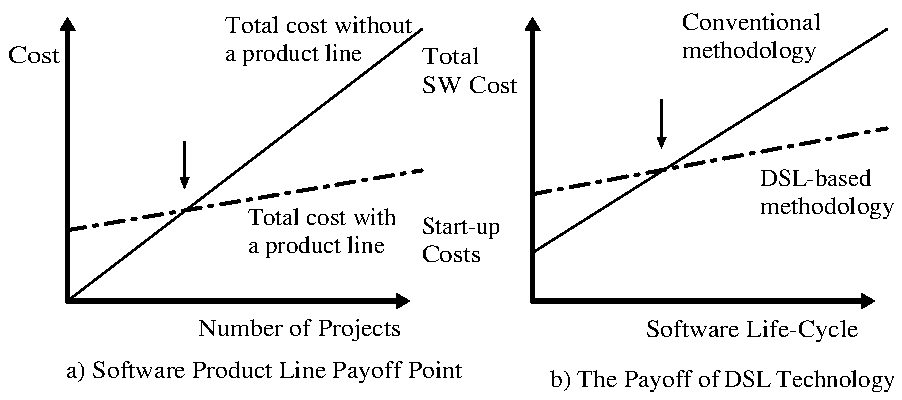
\includegraphics[width=12cm,height=!]{ch02/pl-cost}
	\end{center}
	\caption{Product-Line Payoff}
	\label{fig:pl-cost}
\end{figure}

\begin{figure}[ht]
	\begin{center}
		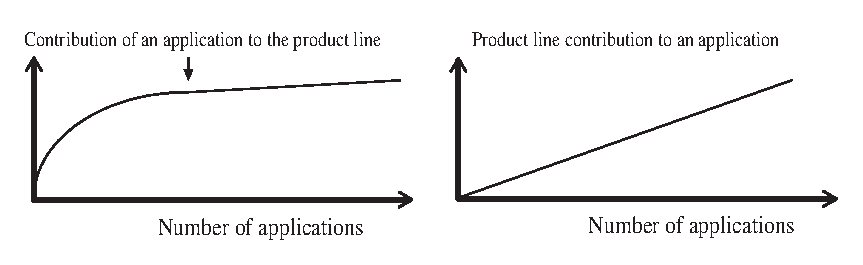
\includegraphics[width=11cm,height=!]{ch02/productline}
	\end{center}
	\caption{A Product-Line and its Applications}
	\label{fig:productline}
\end{figure}

A product-line can be seen as up-front investment that pays itself off in the long term. This is showed often graphically as in case (a) of \fig{fig:pl-cost}, taken from \cite{pl.02}, where the start-up costs of the product-line approach are bigger than those of an approach without a product-line. The product-line investment pays off after a given point. These empirical diagrams look similar for other technologies that require some up-front investment as in case (b) of \fig{fig:pl-cost} that shows the payoff for domain-specific languages (DSL), taken from \cite{hudak98modular}.

An alternative view of a product-line is to consider it as an accumulation of investment, rather than an up-front investment. The more similar applications are built for a given domain, the more the previously implemented functionality will be reused in the new applications. Turning such an accumulation of investment into a really profitable product-line is a matter of discipline and architectural refactoring \cite{refactor.99,sf.04}. There is a mutual contribution between the product-line and a specific application illustrated by the diagrams of \fig{fig:productline}: (a) each specific application contributes (back) to the product-line, enhancing its variability; (b) the factored common product-line functionality is reused with proper variability parameters in a specific application implementation. A product-line is in an iterative development process, while new applications are created for the same family. In the long term, it is expected that after a \textit{threshold} point, the product-line development changes very slowly when new applications are created. The threshold point is envisioned to be very close to the payoff point of the up-front investment view of product-lines.

The iterative view of a product-line is more suitable than the up-front investment view for the domain of mobile device software. Each ubiquitous computing scenario has its own peculiarities and contributes back in the common code base that is shared between all mobile applications, which are based on the same set of technologies for a given domain. The product-line assets are gradually structured as more scenarios are implemented.

\subsection{Variation Mechanisms for Mobile Product-Lines}
\label{sec:var.mob.pl}

The common functionality of mobile applications can be reused when it is parameterized with regard to its variability. There are different mechanisms for organizing and reusing the common product-line functionality, known as \textit{variation mechanisms} \cite{pl.00,harsu.2001}, e.g., component libraries, inheritance and code generation. From the point of view of an iterative approach to mobile software product-line development and evolution, three general requirements can be identified. Some of these requirement are useful for any kind of software product-line, however, they are especially important for mobile applications. 

\begin{itemize}
\item The variation mechanisms for mobile product-lines should \textit{facilitate the introduction and maintenance of domain abstractions.} The creation of a product-line is an iterative process. It should be easy to start creating a product-line, adding functionality to it at any time and maintaining it. No product-line is acceptable unless it can deliver in time \cite{sf.04}. If the costs of introducing reusable assets in a mobile product-line are high, the product-line will not be embraced in the early phases of the development. This will make it even more difficult to introduce a product-line later on, after some applications have been developed. The variation mechanisms should enable the evolution of the domain assets, as the underlying mobile technology (middleware) changes often, to respond to the market demands and technology innovations.

\item The variation mechanisms for mobile product-lines should \textit{enable stating declaratively and introducing automatically the domain functionality.} The integration of the product-line's generic functionality into a specific mobile application should be as much automated as possible. Automation accelerates the time to market, by reducing the debugging time (which is higher for mobile applications because of the indirection gap between the machine where the development is made and the device where the software runs).

The used variation mechanisms should enable a declarative representation of domain assets, in order to preserve the design model within an application, and to avoid accidental complexity \cite{brooks.87}. Declarative constructs are important to ease the maintenance of a product-line during its evolution \cite{Pussinen.2002}, and to clearly define the boundary between the generic domain functionality and the application specific functionality.
%
As noted in the discussion of case (a) of \fig{fig:pl-cost}, the product-line start-up costs are usually higher than the costs of applications without a product-line. Adding the costs of developing a declarative notation (case b), to the product-line start-up costs related to domain engineering, can result in an unacceptable overall cost for a project. As argued in \cite{hudak98modular}, it is not sure that the payoff point really comes in every case. Hence, declarative variation mechanisms with very low start-up costs are needed.

\item The variation mechanisms for mobile product-lines should \textit{enable domain-specific optimizations.} Mechanisms that balance between the increased level of abstraction and the introduced run-time performance are needed. For example, the indirection layers could be minimized. For example, in the J2ME MIDP \cite{www.j2me}, the class meta-data are saved in the application's binary file. The number of classes affects the size of the application and should be kept in a minimum.

\end{itemize}

\noindent To summarize, the variation mechanisms (VMs) for product-lines for mobile applications should:
\begin{enumerate}[a.]
\item make the domain functionality explicit by means of declarative domain specific abstractions,
\item provide for stability of domain abstractions in the prospect of fast underlying technology changes,
\item support automated integration of domain and application functionality,
\item have low start-up costs and require minimal additional (language) technology,
\item enable domain-specific optimizations.
\end{enumerate}

\Kr{ch01} listed several variation mechanisms for product-lines discussed in \cite{pl.levels.00,pl.00,harsu.2001}, e.g., inheritance, code generation, and compiler directives. An overview of the other techniques can be found in \cite{sf.04}. The list of the variation mechanisms given in \cite{pl.levels.00,pl.00,harsu.2001} is extended in this section to include visual modeling and domain-specific languages (DSL), as more declarative mechanisms. The remainder of this section examines OO frameworks, visual modeling and DSL.

\subsection{Object-Oriented Libraries and Frameworks}
\label{sec:ooframeworks}

Object-oriented (OO) libraries and frameworks are interesting variation mechanisms because they enable implementing the domain variability with techniques already found in OO languages. OO libraries are the native way to factor out and reuse functionality in an OO language. The domain variability can be expressed, by using method parameters, overloaded methods, or forms of OO inheritance, e.g., template polymorphism in C++ \cite{cpp.97}.

While OO libraries and frameworks use the same underlying OO language variability mechanisms, the difference between OO libraries and frameworks becomes clear when implementation flexibility is considered. OO libraries allow a lot of freedom in design and usage. The coding and the architectural conventions in an OO library are implicit. It is easy to extend an OO library with new domain assets that do not follow the conventions. The implicit design rules are often not enforced. This results in non-uniform libraries, where the reusable components may follow different design patterns.  Non-uniformity of the design makes it difficult to reuse OO library components in a product-line. It makes also difficult to refactor the product-line as it evolves. Patterns \cite{dpatterns} help to clarify common designs, but they are not a replacement for architecture \cite{patterns2}. It is not uncommon to find more than one different implementation of the same pattern within the same system, resulting from the incoherent design.

In order to access the required domain functionality assembled in an OO library, each application has to go each time through several steps, e.g., component library initialization, object(s) instantiation, selection of required interfaces, and passing of required parameters. This adds accidental complexity to the application code. Component library calls with various parameters are also difficult
to maintain when the library functionality and interface change as the product-line evolves. When domain abstractions are implemented as libraries, e.g., as a library that contains the functionality common to \textit{web ser\-vi\-ces} \cite{webservices.04}, additional classes and interfaces need to be introduced. The more generality is needed, the more indirection the OO implementation will add \cite{webservices.04}. %TODO web service example in code AXIS

Frameworks perform better than OO libraries, when used to organize product-lines. Frameworks place design restrictions in the way the applications are built, and define clear specialization points for the developers to follow \cite{sf.04}. The design restrictions of a framework show in the form of well-defined (a) \textit{specialization} points, e.g., how to create an enterprise bean in EJB \cite{ejb21} by deriving it from a specific priorly-defined based class \see{sec.c2.ejb}, and (b) well-defined \textit{extension} points, e.g., the (missing) possibility to create a new type of bean in EJB. The clear specialization and extension points enforce a uniform structure in a product-line and make it easier for developers of the product-line to maintain it. Developers benefit from the clear specialization points that enable reusing the architecture of the framework in a new application.

Although OO frameworks have been used successfully to organize product-lines \cite{batoryetal.00}, they cannot define proper abstractions to represent the domain concerns, which makes it more difficult to reason about the domain by looking at the code of an application. Using OO frameworks may result in more coding, because the domain variability should be expressed in pure OO language mechanisms. For example, in EJB 2.0 \cite{ejb21} the variability mechanisms are based on OO constructs, such as, interfaces and required method names. The complexity of the programming model in EJB 2.0 motivated the need for EJB 3.0 \cite{ejb30}, which uses a more declarative way to express the domain variability. OO frameworks are not declarative and offer few automation. OO frameworks are often combined with other variability mechanisms, e.g., visual modeling \see{c2.vm} and code generation \cite{generative.00}, that contribute respectively to a more declarative domain representation and more automation. %Nevertheless, the possibility to define clear extension points for the developers to follow is an important feature of the frameworks.

\subsection{Visual Domain-Specific Modeling}
\label{c2.vm}

The most successful approaches in automating embedded software have been those based on visual meta-modeling and code generation from graphical models. Any Computer Aided Software Engineering (CASE) tool can be used to model an application in a domain of interest, and generate code stubs from that model. Visual modeling has been successful for mobile and embedded applications even before the popularity of virtual machine abstractions. The reason is that code generation can be optimized for a given device, and only recently generic virtual machines that run efficiently on small devices could be afforded.

The way CASE tools are used to model software has been gradually standardized under the Object Management Group (OMG)\footnote{\url{http://www.omg.org}}, as Model-Driven Architecture (MDA) \cite{mda.frankel}. The most important standard behind MDA is the Meta-Object Facility (MOF) \cite{www.mof}. MOF defines the structure of a domain in a layered way. The lower layer represents the real information about the objects of a domain, also known as the M0 layer. The next layer, M1, models how this real domain information is represented in a computer. M1 is the lowest practical level for working with a domain. The M2 layer models the data structures used in the M1 level. This is also known as the \textit{meta-layer}, and M2 models are known as \textit{meta-models}.

While M2 is enough to describe any M1 model, often M2 itself needs to be described. The motivation behind this is to enable different M2 representations to be interchanged between different CASE tools. For this reason, at the top of the MOF stands a \textit{meta-meta-model}, known as the M3 layer. The M3 layer is very general and could be used to describe any meta-model, no matter the domain or the methodology the meta-model uses. Because of this generality, the M3 model is hardwired in the MOF standard and no further layers are needed. The M3 model is known as the \textit{MOF model}. Everything in the MOF model derives from a single element, known as the \textit{ModelElement}.

The MOF standard defines the MOF model and various mappings (representations) of the MOF model into various technologies, e.g., UML, CORBA, Java, and XML. The MOF model can be used not only to model data items and relations between them (the \textit{modeling viewpoint}), but also to traverse the model graphs and obtain information about the model (the \textit{data viewpoint}). Both these views are tightly interconnected and are part of the MOF standard. Other standards are currently under standardization by OMG that enable the transformation of the MOF models. While MOF is a generalization of UML\footnote{Unified Modeling Language.} modeling \cite{www.uml}, UML 2.0 will be structured as a special case of MOF. MOF is intended to be a common ground for exchanging models between different visual CASE tools. The ideas behind MOF are quite generic, and MOF can also be applied to textual representations of models, including source code.

%The importance of MDA and MOF does no stand in the model itself, because anyone could come with the same model after a little bit of thinking. The importance stands on the fact that MDA represents set of industry standards. OMG itself is made up of various organizations such standards offer a common minimum agreement between different CASE tools vendors. However most existing CASE tools do not support MOF or support it indirectly as a model of their proprietary meta-meta-models. The reason for this is simple. Functional CASE tools are needed by the industry and on one can wait upon standards to emerge and finalize.

MOF is not directly interesting for domain modeling. Everything can be represented as a MOF model. Such a level of abstraction can be useful to prove theoretical properties of graphs \cite{mens.99}, but only when the models are specialized for a given domain, they become useful in practice. The specific abstractions of a domain are important, because they embody the domain knowledge. They are used to reason about a specific domain better than the generic graph algorithms. The more specific a model becomes, the more useful it is for a given domain. For example, UML profiles \cite{www.uml} enable UML specializations for various domains.

\begin{figure}[ht]
	\begin{center}
		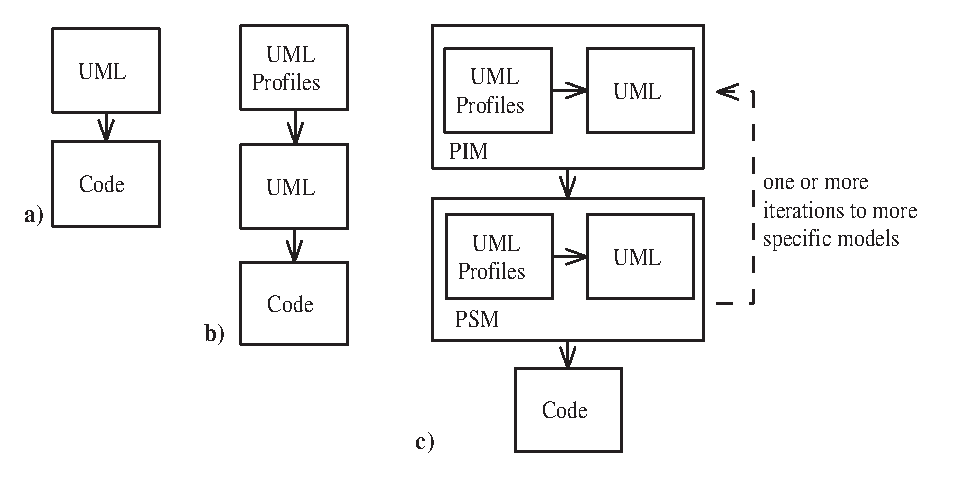
\includegraphics[width=10cm,height=!]{ch02/mda}
	\end{center}
	\caption{MDA Development}
	\label{fig:mda}
\end{figure}

\fig{fig:mda} shows three different ways, how a visual CASE tool can be used to model an application. Although only UML \cite{www.uml} is denoted in the boxes of this diagram, any (meta) model language can be used. The simplest case (a) shows generating code from a visual model which maps directly to the implementation language. Case (a) has been used in the past to generate embedded software. The visual model contains a predefined set of user-defined element classes. Case (a) is usually not very interesting because it supports only an one-to-one mapping into code and hence no automatic injection of the domain concerns is possible.

Case (b) of \fig{fig:mda} uses custom additions to the generic meta-model, in this case through one or more UML profiles, which helps to factor out and to reuse the domain functionality. For example, the UML profile for Enterprise Java Beans (EJB) \cite{www.uml.ejb,www.uml.ejb.omg} \textit{"defines a set of UML extensions that capture the structure and semantics of EJB-based artifacts"} \cite{www.uml.ejb}, mainly by utilizing stereotypes and typed values. The EJB profile captures the semantics of a specific domain, in this case of EJB \cite{ejb21}, in the form of predefined profile entities that can be reused to model applications in this domain. Rather than having to define applications in terms of object-oriented (OO) classes, a designer relying on the EJB profile can directly use EJB concepts, such as, \flqq{}EJBEntityBean\frqq{} or  \flqq{}EJBPrimaryKey\frqq{}. Case (b) represents how most existing CASE tools work.

The third case (c) generalizes case (b) by splitting the transformation of a model to code into several configurable transformation steps to intermediate models. Case (c) stands for the generic MDA scenario, where the created model (known also as \textit{Platform Independent Model} - PIM) is refined into a more specific model (\textit{Platform Specific Model} - PSM), before some executable equivalent is generated. This could require more than one iteration, moving to a more specific model in each iteration, whereby each model uses its own specialized profile. The case (c) implies also that the details of the PSM are automatically inserted into the PIM using appropriate transformations. While case (b) can be used for a product-line, it is the automated model of case (c) that could be of most interest for automated product-lines that require more than one mapping step, in order to postpone some of the design decisions to a latter phase. That is, case (c) supports \textit{progressive refinement} \cite{sf.04} of the application architecture, from a very abstract design model to more specific models, known also as a stratified design \cite{kuhne.03,kuhne.01}. %Case (c) automatically reduces the architectural gap between the product-line abstractions and the implementation of specific applications.

There is no agreement in the MDA community on what is the best way to define PIM to PSM transformations. Often, only the structure of a model is defined graphically in a CASE tool, that is, components, their interfaces and relations. Although it is possible to define method implementations graphically (e.g., by using UML Actions), in practice it is often easier to associate pieces of code directly with the structural model elements, which means that pure visual models are rarely used.

An example of a commercial meta-modeling tool, used to model mobile and embedded software, is MetaEdit+ \cite{MetaEdit.Home} from MetaCase. MetaEdit+ has been used in several Nokia \cite{www.nokia} projects, e.g., graphical user interface modeling for TETRA (TErrestrial Trucked RAdio) devices \cite{MetacaseCase.03}. The main rationale behind MetaEdit+ is that domain-specific visual languages and visual domain-specific abstractions help to automate software development \cite{metaedit.embedded}. MetaEdit+ enables the creation of meta-models for specific domains, and using the elements of these meta-models to model specific domain problems. The domain elements and their relations are presented graphically. Source code artifacts can be associated with parts of interests, and various predefined or customized reports (including source code) can be generated from the models. Model transformations are not supported directly in MetaEdit+, and it basically works based on the model of case (b) of \fig{fig:mda}. 

Another example of a CASE tool is the Generic Modeling Environment (GME) \cite{gme.01}. GME, like MetaEdit+, uses a proprietary meta-meta-model and offers limited support for MOF, as just another meta-model. GME is a university research tool, developed based on the concept of Model Integrated Computing (MIC) and MultiGraph Architecture (MGA) \cite{gme.mic}. While the terminology used in the GME documentation is sometimes peculiar, most of the MGA concepts can be directly mapped to the MOF terminology and MGA could be considered to be a custom case of MOF. % as shown in Table~\ref{tab:GMEMGAVsMOFTerminology}.

Compared to MetaEdit+, GME is limited only on defining meta-models, model constraints\footnote{The UML Object Constrains Language (OCL) is used.}, and graphical models based on these meta-models. Code generation or other reports should be implemented as Visual C++ add-ins, or generated by doing a traversal of the model graph, by using various script languages that can access the GME COM components API. The transformation of the models is supported via graph transformations \cite{gme.graphs} using other tools outside GME. Graph transformations support the case (c) of MDA development of the \fig{fig:mda}. Graph transformations are based on writing transformation (graph rewrite \cite{schurr.graph.94,Blostein-Schuerr02:99}) rules as left-hand and right-hand side subgraphs. The left-hand subgraph, when found in a graph, is replaced with the right-hand subgraph. The specification of rules can be done graphically in a CASE tool, e.g., GME, or by using more formal grammar rules \cite{Rekers-Schuerr02:97}.

Matching of the left-hand side rules in a graph can be simplified by sequencing the order in which the rules are applied \cite{gme.graphs}, or by restricting the form of the left-hand side of a rule \cite{Rekers-Schuerr02:97}. Rule matching can also be simplified by starting on predefined nodes, known as part of the sequence rules for a given domain. Milan \cite{gme.milan} is a framework based on GME, for the simulation of embedded system designs, in particular System-on-Chip (SoC) designs. Apart from GME modeling components, Milan also supports various simulations of the designed systems, using other third-party software. Another GME based system is GRATIS \cite{gme.gratis}. GRATIS supports high-level visual modeling for TinyOS \cite{gme.tinyos}, a small operating system for embedded devices. GRATIS helps to manage the event-based component communication in the TinyOS, reducing the development errors that result from directly maintaining the component interaction files.

Some other approaches, such as, SmallComponents \cite{www.smallcomps}, use predefined UML profiles to generate the entire OS required in an embedded device, by including only those parts that are interesting for an application. Small\-Components-like approaches can be useful for small embedded devices where the entire system is generated at once containing a set of selected predefined applications. A comprehensive list of existing CASE tools can be found in \cite{case.tools}, whereas a list of preferable features for such tools can be found in \cite{uml.tools.criteria}.

Based on the criteria for mobile product-lines listed in \sr{sec:var.mob.pl}, there are several reasons why visual modeling in isolation is not very useful as a variability mechanism.

\begin{itemize}
\item \textit{Partial automation}. Ideally, a visual model can be used to generate code in more than one target language. The final target code is, thus, not very important to a CASE tool. In practice, this requires that the entire functionality is defined visually, which is not preferable in complex application domains, where a lot of specific application functionality must be coded manually. For this reason, CASE tools can easily generate stubs of code for a language, but leave most of the method implementation details to be filled out manually. Various techniques \cite{voelter.generation}, e.g., the template method pattern \cite{dpatterns}, can be used to keep the manually added code separately from the generated code.

\item \textit{Difficult evolution}. Creating product-lines is an iterative process. The domain abstractions are not known from the beginning and they normally evolve as the product-line matures. The final generated code for such abstractions may not be optimal, or completely known from the beginning. Maintaining evolving abstractions visually in a CASE tool could result in additional costs \cite{lop.94}, because the meta-model and all the models based on it must also be maintained.

CASE tools are better suited when the domain abstractions are nearly frozen and well-known. Language abstractions can better support iterative development of product-lines if their implementation and maintenance costs are low. Once the product-line stabilizes, it is usually easy to map domain abstractions, implemented by the programming language(s), to visual modeling elements.

\item \textit{Loss of design information}. Another issue using CASE tools alone, without appropriate support at the language level, is that source code is treated as an end product, similar to the binary code generated by a compiler. Despite comments added by a CASE tool in the generated code it is difficult, or impossible, to preserve the visual model architecture in an easy understandable way. It could be argued that the source code is not important, as long as the model is present. The model hides the details of the code that are not important for a domain. However, given that code must be often edited or completed manually, it is difficult to follow changes and debug it. %Often, CASE tools offer only one way transformations, from model to code, but cannot completely reverse engineer any meaningful design from the code \cite{riel.96}. 
Domain-specific abstractions, when supported directly at the programming language level, help to bridge this architecture gap.

\end{itemize}

\subsection{Domain-Specific Modeling with Language Abstractions}
\label{sec:var.dsa}

This section discusses ways to support domain-specific modeling with language abstractions, rather than with visual abstractions and CASE tools. \textit{Domain-specific abstractions} (DSA) refer to abstractions that are added to, or directly supported by a language, or that are an inherent part of the language, in order to support domain-specific modeling. For example, in the domain of web services special keywords, such as, \texttt{webservice} and \texttt{webmethod}, could be used to denote special treatment of web service constructs by the compiler, e.g., to automatically generate WSDL\footnote{Web Service Description Language. (http://www.w3c.org)} files. Such keywords can be used to define a \texttt{TravelAgent} class, as a web service component, as illustrated in \fig{fig:webservice-dsl}.

\begin{figure}[ht]
\begin{center}
\begin{minipage}{7cm}
\begin{scriptsize}
\begin{lstlisting}[numbers=left,language=Java,frame=leftline]{}
webservice TravelAgent {
  ...
  webmethod GetHotels(){...}
  ...
}
\end{lstlisting}
\end{scriptsize}
\end{minipage}
\end{center}
\caption{A Domain-specific Extension to Implement Web Services}
\label{fig:webservice-dsl}
\end{figure}
 
\noindent There are several benefits from using declarative DSA as a variation mechanism for mobile product-lines:

\begin{itemize}
\item \textit{DSA preserve the architecture of the domain in source code.} Consider the example of the web service abstraction (\fig{fig:webservice-dsl}) as a part of a product-line. When web services are supported declaratively in the language, a single keyword \texttt{webservice} can be used in every place the web service functionality needs to be reused. The source code with the declarative domain abstractions is easier to understand. The code is not considered as the end-product of some generator, which is difficult to modify by hand, but as a means to express the domain design. DSA help to trace the architecture down to code, as well as, to reconstruct the architecture from source code \cite{sf.04}.
%
DSA support automation and reduce accidental complexity\footnote{Complexity related to the particular solution, not inherent in the solved problem itself. The later is known as \textit{essential complexity} \cite{brooks.87}.} in a product-line. While DSA have the same explicit programming model as OO libraries \see{sec:ooframeworks}, they automate the instantiation and usage of the domain abstractions in source code.

\item \textit{DSA can be used as an alternative to visual modeling.} It is easy to support a set of DSA, that are in place for a domain, with CASE tools. For example, an icon in a CASE tool can represent a \texttt{webservice} which will be mapped directly onto the corresponding DSA construct in the source code. Declarative DSA blur the distinction between an explicit modeling step, and directly modeling at the source code level. 
Working directly with the code, to refactor it using DSA, reduces one step in going through a visual modeling tool, but at the same time supports the same level of abstraction. %This can be beneficial, because the proper code abstractions may not be known right from the beginning. 

\item \textit{DSA implementations can be optimized using generative techniques.}  The DSA processing tools have access to the abstract syntax tree (AST), and can directly inject the domain code into the AST locations where the DSA are found. To the end user, the abstractions are still declarative. It is hard to achieve this with object frameworks \cite{dsl-pl.2000, batoryetal.00}, where OO inheritance and composition are exclusively used.

\end{itemize}

\noindent There are several ways to support DSA:

\begin{enumerate}[i.]
\item New languages can be defined from scratch, whose elements directly correspond to abstractions in a particular domain. Such languages are called \textit{Domain-Specific Languages} (DSL) \cite{deursenetal.00}. For example, Maple\footnote{http://www.maplesoft.com/} is a computer algebra system specialized for calculating specific mathematical formulas. Such specialized languages are very effective in some domains. However, often it makes sense to reuse as much of an existing host language as possible when adding DSA.

\item \textit{Embedded Domain-Specific Languages} (EDSL) integrate DSA into a host language \cite{leijen.99,kamin.98}. The host language is often a general-purpose language, e.g., Java, which is augmented with declarative constructs to support one or more domains of interest. An example of an EDSL, is SQLj \cite{www.sqlj}, an embedded SQL engine for Java.

\item Another way to support DSA is indirectly via \textit{general-purpose software abstractions}, which are first added to a host language in order to (a) make it  extensible to support EDSL-like constructs, or (b) to support generic meta-modularization\footnote{These generic modularization mechanisms need to access the meta-model of a language to enable factorizations that are not possible with inheritance and composition alone.} mechanisms not found in the original language. An example of an general-purpose software abstraction for supporting extensibility is the support for \textit{attributes} in .NET \cite{www.dotnet}, or \textit{annotations} added recently to Java. An example of a generic meta-modularization mechanism that can be used to support EDSL is \textit{Aspect-Oriented Programming} \cite{kiczalesetal.97} as supported, e.g., by AspectJ \cite{www.aspectjt,Laddad.aop} \see{ch2:aop}. The general-purpose software abstractions are not specific to any particular domain and can be used to support several EDSL within the same host language.
\end{enumerate}

\noindent In the following, several drawbacks are discussed, which prevent DSA supported by the first two alternatives (DSL and EDSL) from being widely accepted as a variability mechanism for product-lines. Attribute-based DSA are discussed in \sr{c2.sec.dsa.attributes}, while AOP-based DSA are explained in \sr{sec.aop.dsa}.

\begin{itemize}
\item \textit{High start-up costs}. DSA realized with the first two approaches have the highest start-up costs compared to other variability mechanisms, e.g., component libraries, and require careful planning of the expected variability. Adding the DSL start-up costs \cite{hudak98modular}, schematically shown in case (b) of \fig{fig:pl-cost}, such as defining grammar extensions and interpreting declarative
constructs, to the product-line start-up costs devoted to domain engineering \cite{harsu.2001} and variability representation \cite{harsu.2001}, may result in an unacceptable payoff point for a product-line. This motivates the need for technology that reduces the DSL introduction costs in iterative product-lines.

\item \textit{Difficult to evolve.} DSA are also difficult to maintain in order to support product-line evolution. As with every software system, it is very probable that the proper declarative abstractions cannot defined clearly from the beginning. The development is more iterative in the early phases of the product-line. The cost of changing DSA is usually higher than, e.g., that of maintaining libraries or object frameworks. The implementation of the abstractions and their representation needs to be modified, which affects the language grammar and its parsing. The DSA technology should support experimentation during the iterative product-line development.

\item \textit{Accidental costs.} DSA frameworks introduce additional costs not only for implementing the DSA itself, but also for educating the developers to use the abstractions. Last but not least, DSA introduce unnecessary external dependencies of the product-line on third-party frameworks, needed to implement the DSL additions, which may increase the product-line maintenance costs in the long term. There is also a lack of standard parsing tools and DSL supporting API-s in languages, which renders the implementation of reusable DSA difficult. The DSA technology should be part of the programming language supported by the language vendor.

\end{itemize}

%The reason we treat all of these language abstractions in a single group is that the mechanics for implementing them are more or less the same usually resulting is some transformation of the program abstract syntax tree (AST). Program transformation \cite{www.pt, dms.02} can also be used alone without a DSA front-end, in form of program generators.  Several generative techniques exist \cite{generative.00} , where the variability parameters of a solution are used to drive the generation process. Using parameterized code templates\footnote{By template here is meant any parameterized piece of code (by some means), not only C++ templates. Frame based approaches, and other more exotic approaches, such as, framed aspects \cite{framed.aspects} fall also into this category.} and code snippets can shorten up development time of generative solutions. However, generative techniques, when used alone, lack a declarative support for domain abstractions and make it difficult to preserve the domain architecture into the source code. For a compressive overview of such techniques refer to \cite{generative.00}.

\section{Software Containers}
\label{c2sec:containers}

\Kr{ch03} shows how attribute-based DSA can be used as a low-cost DSL alternative to represent domain concerns in source code. Selecting a variability mechanism is not enough to create a product-line. A structured way to organize the domain assets of the product-line is needed. An \textit{architectural abstraction} \cite{harsu.2001} could be combined with one or more variability mechanisms, in order to support product-line creation and evolution. The product-line architecture \cite{harsu.2001} defines and enforces an implementation methodology to represent and to organize the product-line assets \cite{pl.02}. For example, when OO inheritance is used as a variability mechanism, a well-defined hierarchy of the domain assets could be created.

The product-line architecture should define clear extension points for the developers that extend the product-line \see{sec:ooframeworks}. The DSA constructs are connected with the domain assets implemented in the form of OO libraries \see{dsa.connect}. However, when the DSA become easily to implement, there could be a lot of unstructured DSA constructs added to support the product-line. The unstructured DSA interpretation can become a bottleneck for the product-line evolution.  

Several architectural styles \cite{harsu.2001} have been explored for product-lines, e.g., data-flow architectures and virtual machine architectures \cite{harsu.2001}. The interest in this book is (a) in low-cost mechanisms that support the iterative view of mobile product-line development and (b) in automated reuse of product-line assets in specific applications. Following the current trend of component-based development \cite{comp.soft.book}, supported by today's general-purpose OO languages, such as Java and .NET, this book focuses on component architectures \cite{otm,comp.soft.book,comp.soft.book2,assmann.99-comparison} based on \textit{software containers}. Containers place a clear distinction between the domain functionality, organized as low-cost DSA, and the rest of the application specific functionality. %As this section explains, software containers help both with structuring and with the automatic reuse of the product-line assets.

The container abstraction is usually related to server-side enterprise container implementations, e.g., COM+ \cite{comp.services} and EJB \cite{j2ee14}, and could be described by a combination of software patterns \cite{server.patterns.02}. The container abstraction can be used to organize product-line assets for any application domain. A software container serves as a high-level architectural abstraction, used to organize common domain functionality as services and introduce them nearly transparently to an application\footnote{Unlike most real-world containers, a software container offers some kind of support (services) to the object found in (managed by) it.}. This section starts with an overview of two existing enterprise container implementations, COM+ and EJB. The remainder of the section explains how containers can be used in arbitrary domains, and why is it beneficial to use them to organize mobile product-lines.

\subsection{Microsoft COM+}

COM+\footnote{The term COM+ is used here synonymously with Microsoft Transaction Service (MTS).} \cite{comp.services,www.comp} is one of the first wide-spread enterprise containers. It uses an underlying component model based on Microsoft DCOM\footnote{DCOM stands for Distributed COM, whereas COM itself stands for Component Object Model. Both are proprietary component models.} \cite{www.dcom} technology, which allows components to reside nearly transparently in any networked machine. COM+ is mainly intended to facilitate implementation and maintenance of big enterprise applications. Some of the COM+ services, e.g., catalogs, that organize and maintain sets of components, can be used to support any distributed application. A COM+ application can be configured either programmatically, using any (script) language that can access COM objects, or via GUI tools.

A COM+ application consists of two types of DCOM components: (a) \textit{serviced} components that use the services offered by the COM+ container, and (b) \textit{client} objects that interact with the serviced components. Each COM+ component has its own identity and can be manipulated individually if needed. The idea behind COM+ (as with any container) is that application components that use the COM+ services, are developed by leaving out the exact details of service configuration to COM+. The following discussion of COM+ services is based on \cite{comp.services}.

One of the basic services offered by COM+ is a fine-grained security model based on \textit{roles}. Each role has a well defined set of permissions that specify, which components and component resources, e.g., databases, the role is allowed to access. Users are assigned to roles and this determines their permissions.

Transaction management is another service offered by COM+. A transaction is a sequence of operations that is treated as a single logical operation, and enjoys atomicity, consistency (in the terms of invariants), isolation (no side effects), and durability (introduced changes are not lost). The underlying DCOM technology supports distributed transactions relying on a distributed two-phase commit protocol \cite{Coulouris.01}. Users can also define custom atomic resources, using Compensating Resource Manage (CRM) service, to allow any kind of created or acquired resource to take part in a transaction.

COM+ helps to manage the internal state of component instances by distinguishing between \textit{stateless} objects, \textit{cached state} objects, and \textit{persistent} objects. The internal state of stateless objects is not important and does not need to be preserved. The cached state objects can have their state preserved while the application is running in a shared property manager (SPAM)\footnote{Shared Property Application Manager.}, indexed by string keys. The state of persistent objects can be stored in persistent storage directly or in a relational database. 

Object state is related to object life-cycle management. COM+ manages the life-cycle of objects in order to transparently support scalability\footnote{COM+ can also handle load balancing by distributing requests in a cluster of several machines.}. To handle a large number of sporadic clients for an object, COM+ uses Just In Time Activation (JIT). JIT creates an object instance only when it is needed, and passivates it during the idle time to save the system resources. This service is complemented by object pooling, where several instances of a component are kept and reused to re-personify\footnote{This is similar to \textit{virtual instances} in Java EE \cite{server.patterns.02}.} serviced objects every time a specific object is needed by a client. To achieve pooling, a client does not use COM+  objects directly, but via a \textit{moniker}, which is a DCOM abstraction of an instance handle. A moniker can be used to represent any resource. Database connections are also COM objects, so they can be pooled using the same mechanism too.

An important feature for an application is the ability to synchronize its own activities. COM+ deals with synchronization by supporting different threading models known as \textit{apartments}. A component is activated (invoked) always within a specific thread model. The apartment model is specified when the component is deployed in a COM+ application by setting the right apartment type as part of the configuration. Access to multi-threaded apartment (MTA) objects is synchronized by COM+. A related COM+ concept is an \textit{activity}, which represents a set of objects that are used by a single client (similar to a session). Synchronization can also be controlled at the level of the individual activities.

Another related service is Microsoft Messaging Queue (MSMQ), a pu\-blish-sub\-scribe event service often used by COM+ applications. MSMQ can be used alone without COM+, but it is often used for asynchronous message-based object invocations inside COM+. COM+ applications can also use lightweight directory services\footnote{Lightweight Directory Access Protocol (LDAP).} to locate resources and other components via Microsoft Active Directory service.

One of the problems with using COM+ in the past has been its complex programming model \cite{www.comp}. This complexity comes from the fact that DCOM and COM+ add several layers of abstraction, while preserving the underlying details. COM+ \textit{serviced} components are DCOM components, usually written in C++. DCOM introduces an interface declaration language (IDL) and several implicit programming conventions. COM+ adds another layer of explicit and implicit conventions to DOM that must be known and followed to use COM+ successfully. The preservation of all these details of the programming layers made sense back in the early days of COM+ when the technology was not mature. It was useful to be able to experiment with the technology in order to understand the properties of its abstractions and their implementations. Having access to the implementation details enables also manual optimizations for software that has to run in slow machines. Such a detailed programming model with little automation can work only for relatively few and small applications.

In last ten years the situation has quickly improved. As the computer hardware becomes much cheaper than software and there are faster machines, there are also more and larger applications. Language-based abstractions, such as those of .NET \cite{www.dotnet} language families, supported by virtual machines are not considered slow anymore. Long experience with COM+ and DCOM have revealed the repeated coding idioms that could be abstractions on their own. With .NET, \cite{www.dotnet} Microsoft introduced a new, simpler and less restrictive programming model for DCOM \cite{clr.com} and COM+ \cite{com.dnet}, based on meta-data and explicit attributes. The COM+ support in .NET is part of the \texttt{Sy\-stem.Enter\-pri\-seSer\-vi\-ces} namespace \cite{com.dnet}.

\subsection{Java EE and Enterprise Java Beans}
\label{sec.c2.ejb}

Similar to COM+, Java Enterprise Edition (Java EE) \cite{j2ee14} is a container-based technology for enterprise server-side applications. Java EE is based on Enterprise Java Beans (EJB) \cite{ejb21} component model, relying on Java \cite{www.java} component model (beans and remoting)\footnote{These are also proprietary component models.}. Unlike DCOM, the Java component model is simpler to use. Java itself (unlike C++) belongs to the family of languages that maintain meta-data as part of their binaries\footnote{The Java binaries (*.class files) are actually pseudo-binaries that require a virtual machine to be interpreted and cannot be executed directly.}. This simplifies the programming model, e.g., the discovery of the interfaces implemented by a component, is directly supported by the language. Java technology (and Java EE) is an example of the second wave of enterprise containers and technologies used to build them, where more abstraction layers can be afforded as the hardware becomes faster.

While Java EE and COM+ (MTS) offer more or less the same set of services, the terminology is often different. Java EE, for example, uses the term \textit{role} to denote different stages of an application development and life-cycle, e.g., enterprise bean provider, application assembler, deployer, container provider, whereas COM+ does not define any specific terminology for the developer roles. The components are called \textit{beans} in Java EE.

The programming model for the container services is different too. Java EE distinguishes between various types of beans, such as, stateless, session, entity (persistent), and message-driven (event based). Unlike COM+, where the stereotype of a component is specified as part of its configuration attributes, in Java EE components state their type explicitly based on required interfaces specified as part of their implementation and other implicit\footnote{That is, many Java EE component coding rules are not part of the language syntax and cannot be enforced explicitly by the Java compiler.} coding rules, e.g., required method names.

Services offered by Java EE include, for example, security, transaction management, naming, message-based communication and timer service. There are slight differences between these services and the corresponding COM+ services. For example, security in COM+ is not concerned with user authentication, since this is handled by the operating system, whereas Java EE deals with user authentication itself, because it is intended to work in multiple different server operating systems.
Naming (JDNI) in Java EE corresponds to Active Directory services in COM+, whereas message-based communication via message-driven beans is similar to MSMQ. A Java EE bean can use the timer service to register callbacks to be called at a given time or periodically. The timer counters are persistent and callback registration can be treated as a transactional resource (as with CRM in COM+). Object pooling and database connection pooling are also handled by Java EE. Java EE uses the term \textit{virtual instances} \cite{server.patterns.02} for handles to the pooled objects (in COM+ a handle is implemented by a moniker).

The most interesting aspect of Java EE is the evolution of its programming model. EJB, up to version 2.1 \cite{ejb21}, makes use of required interfaces and pseudo-syntactic rules (coding conventions), such as naming rules for method names. Creating a bean implies defining one or more required interfaces. Furthermore, beans that need some form of life-cycle management, must implement required callback methods, e.g., \texttt{ebjActivate()}. Most of these actions are repeated with few variations and could be automatically generated. It is unclear why EJB did not define from the beginning proper abstractions, to deal with such tedious programming tasks, that can be easily automated and made transparent\footnote{When EJB appeared its programming model was significantly easier to use compared to COM+. The .NET programming model for serviced components is now simpler than EJB.}. Third-party tools, e.g., xDoclet \cite{www.xDoclet}, appeared to deal with such inconveniences of the EJB programming model.

EJB is also moving toward a simpler programming model, based on attributes \cite{java.explicit.programming}. The latest EJB specification \cite{ejb30} uses predefined attributes to decorate component implementations, which are now \textit{plain old Java objects} (PoJo-s) with very few implicit coding rules.

\subsection{Using Containers Beyond the Enterprise Domain}
\label{c2.container.domain}

Since the term \textit{container} was made popular by COM+ \cite{comp.services} and EJB \cite{j2ee14}, many people use the term synonymously with enterprise containers. Enterprise containers, such as, COM+ and EJB, are often referred to as \textit{heavyweight containers} \cite{aspectComp.03}, which means:
\begin{enumerate}[a.]
\item COM+ and EJB are container implementations for a hardwired problem domain. The containers are defined exclusively for enterprise server applications, usually involving relational databases as back-ends. These container implementations cannot be reused in other domains.
\item Even for the enterprise domain, COM+ and EJB containers offer only a predefined set of services. EJB and COM+ containers cannot be easily extended to introduce new kinds of services into the domain \cite{aspectComp.03}.
\end{enumerate}

Heavyweight container implementations are tightly coupled with the specific problem they solve. The container as an abstraction is domain independent and open to accommodate new kinds of services. In particular, the container abstraction can be used to conveniently implement automation of application families (product-lines). The functionality offered by a product-line (the reusable assets of the product-line) can be seen as a set of services offered by the product-line container abstraction. The specific application components managed by the container (managed components), known also as \textit{serviced components} \cite{com.dnet}, use the container services as shown in \fig{c2fig:container}. The container service variability parameters are given as part of the deployment specification of an application component in the container. The variability parameters are shown in \fig{c2fig:container} in the form of a deployment interface. The actual implementation may vary depending on the container. The serviced components use the services provided by the container. The connection between the container services and the serviced components is known as \textit{service injection} \cite{com.dnet}.

\begin{figure}[ht]
	\begin{center}
		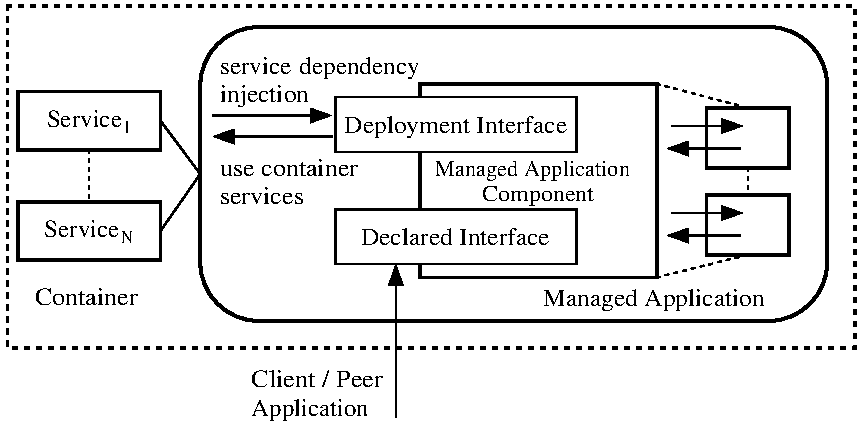
\includegraphics[width=12cm,height=!]{ch02/container}
	\end{center}
	\caption{The Container Abstraction}
	\label{c2fig:container}
\end{figure}

The container abstraction enables a uniform treatment of the services modeling the assets of a specific domain, and the generic services modeling cross-cutting concerns \see{ch2:aop} that may be shared by many applications of different families. The developers of a product-line can manage generic concerns, such as data persistence, within the same container framework as the specific assets identified in a particular domain, e.g., image adaptation required by mobile image processing applications. The container abstraction enables the organization of an \textit{extended} view of a product-line (\fig{c2fig:extended-pl}), whose assets include generic concerns used in the same way, as the assets of a specific application family. An extended product-line is made up of more specific intersecting sub-families that share common assets with each-other, having a network of domains \cite{generative.00}. The shared set of services is represented by the intersection of the different sub-family (assets) eclipses in \fig{c2fig:extended-pl}. The generic concerns are needed by most of the application sub-families within the extended product-line, whereas the application family specific assets are needed only within a family of applications. The uniform treatment of the services enables better share and reuse of the specific services developed for a family, in another family or set of such.

\begin{figure}[ht]
	\begin{center}
		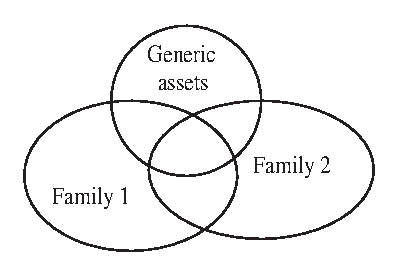
\includegraphics[width=5cm,height=!]{ch02/extended-pl}
	\end{center}
	\caption{The Extended Product-Line}
	\label{c2fig:extended-pl}
\end{figure}


Using the container abstraction to organize a product-line, increases the transparency of reusing the domain services, and results in a better separation of concerns \cite{parnas.72}, because of:
\begin{itemize}
\item \textit{Inversion of control.} The container provides a software indirection for injecting dependencies. The \textit{dependency injection} pattern \cite{fowler.ioc.04}, also known as \textit{inversion of control} (IoC)\footnote{IoC is also expressed as the \texttt{Hollywood Principle}: \textit{"Don't call me, I'll call you."} \cite{spring.article.03}. See \cite{fowler.ioc.04} for a discussion as why the term \textit{dependency injection} is preferable to IoC.}, implies that a component does not explicitly obtain the services it needs but rather, declares its dependency on them by following certain conventions. The declared services are then provided transparently to the component, as necessary, by the environment \cite{lorenz.96,ea.05}. Dependency injection \textit{"moves the responsibility for making things happen into the framework, and away from application code"} \cite{spring.article.03}.

The container connects the product-line services and the application-serviced components in a transparent way. When a service component library is used directly, the exact interface of the service components should be known to the application and be referenced explicitly \see{c2sec:implement}. This is problematic, not only when the interface of the library changes, but also when the library is maintained and several versions of it appear. When inheritance is used, e.g., in a framework, the fragile base-class problem can be encountered \cite{Mezini.97,comp.soft.book,Nathanael.04}, as the base classes evolve. The container abstraction separates the need for a service, from the need to explicitly reference the implementation of the service. The exact service references are introduced transparently to the managed application component.

\item \textit{Improvement of modularization.} The concerns addressed by a product-line are often of a cross-cutting nature. They involve functionality that is needed in more than one place in an application, and negatively affect the overall modularization \cite{Crosscutting1.03,Crosscutting2.03}. The transparent dependency injection, offered by the container, allows developers to focus on those concerns that are specific to application components. The cross-cutting service concerns of the product-line are then introduced automatically by the container. %With a container it is easy to keep the concerns separated in any point in the future, because application components implementation is stored before it is deployed in the container, not after it.

\item \textit{Automation of the development process.} The container abstraction automates the development of applications in a product-line. Product-line automation significantly decreases the development and maintenance costs. The maintenance is improved because the container offers a centralized point to isolate specific middleware services from an application. The container abstraction offers a structured and centralized \textit{object transaction monitor} (OTM) \cite{otm}. This makes it easier to maintain and port mobile application families when the underlying middleware changes.

\item \textit{Implementation architecture.} The container abstraction is a high-level architectural abstraction. It does not replace the usual techniques for product-line implementation, e.g., libraries and code generation. It rather serves as an umbrella for all possible technologies that can be used. One or more technologies can be combined together, to implement the container abstraction in a way that is convenient for a certain domain. %The container places a clear structure on the ways these technologies are used to introduce well-known domain services into a specific application.

\item \textit{Separation of developer roles.} As stated in the Java EE specification \cite{j2ee14}, the container abstraction helps to divide developers in clear distinguishable categories, according to the application development roles: (i) developers that implement the container functionality; (ii)  developers that implement services for the container; (iii)  developers that implement managed applications using the container; (iv) developers that deploy the managed applications into the context of a container. These roles are clearly distinguishable and could be used to properly structure all developers that work with a product-line in an organization.

\end{itemize}

\noindent The container automation has also a few drawbacks depending on the implementation:
\begin{itemize}
\item \textit{The need to learn new coding conventions.} Explicit or implicit coding conventions must be followed by a component implementation if it is going to be used inside a container. These conventions should be learned and properly used by the programmers. For example, an object of a managed virtual instance \cite{server.patterns.02} must not contain methods that return the \texttt{this} pointer directly. This coding convention is required, because otherwise a client would always obtain a different physical reference to the same logical object.

\item \textit{No specialized language support for the coding conventions.} Cheeking implicit coding conventions automatically may be difficult. Explicit coding conventions can be automatically checked, but must be introduced and learned. Explicit coding conventions could be in the form of required interfaces, e.g., \textit{EJBMessageBean} in EJB \cite{ejb21}, or based on some form of DSA, e.g., using additional keywords. Implicit coding conventions are harder to check automatically than the explicit coding conventions are, but require no special syntax to be supported.

\item \textit{Traceability problems because of indirection.} Another related problem is testing and debugging. The indirection introduced by the container makes it difficult to understand the overall functionality of a managed component. This makes it more difficult to debug and test the implementation of the managed components. Nevertheless, debugging can be supported with proper tools and built-in container support for traceability \see{sec.tango.trace}.
\end{itemize}

\subsection{Mobile Containers}
\label{c2.mobile.container}

This book introduces the use of containers to organize mobile software product-lines for J2ME MIDP \cite{www.j2me,www.midp} \seec{ch05}. The container abstraction needs to be specialized in order to reflect the characteristics of the MIDP \cite{www.midp} domain. The mobile software is usually a combination of server-side software and client-side software on the mobile device. Because of limited capabilities of mobile devices, it is desirable to execute as much of the application functionality as possible on the server-side. Ideally, mobile applications should be thin clients. This is not possible for most mobile applications, because a mobile device usually has only sporadic network connectivity. The mobile applications should be able to function even when no network connectivity is available, or to keep at minimum the on-line time, to reduce the connection costs.

Support on the server-side is also needed for mobile applications. For example, images need to be resized to adjust their resolution (or HTML pages need to be converted to WAP \cite{www.wap} format, in a WAP-portal), before they are sent to a mobile device. The data need to be prepared on the server-side, before are sent to a mobile device. Data adaptation can be done transparently from the rest of server-side applications, by using some form of the adaptive-proxy pattern \cite{fox96adapting}, before the data are sent to a mobile device application.

To address mobile software product-line issues, this book introduces the notation of a \textit{mobile container}, which is a special kind of container for managing mobile client applications \seec{ch05}. A mobile container helps to organize services needed by a mobile client application and can be used to support product-lines for mobile applications. The implementation of the offered services is split into a server-side part, and a client-side part running on the mobile device. The client-side implementation must be optimized to reduce the number of abstraction layers resulting from the container indirection. For a managed application running on the mobile device, the container services are transparent. It is the container's responsibility to coordinate the client and the server parts and to provide the requested services to the client applications.

\Kr{ch05} elaborates more on how mobile containers can be structured and about the technology that can be used to build open \textit{container families}, which can be customized to support product-lines for more than one domain. The container implementation introduced in \kr{ch05} is based on a generic Java-based framework, and is open for adding new services for arbitrary domains. The implementation is then specialized with a set of service plug-ins for J2ME MIDP \cite{www.j2me} applications.

\section{Container Implementation Techniques}
\label{c2sec:implement}

%The container abstraction can be implemented using any of the variation mechanisms described in this chapter, e.g., visual CASE tools (UML profiles), or DSA. As noted in sections~\ref{sec:var.mob.pl} and~\ref{sec:var.dsa}, declarative language support for architectural abstractions, such as containers, helps to preserve the design of an application in its source code. However, introducing and maintaining DSA abstractions is often costly. For this reason, container developers have explored various techniques. Some of these techniques try to employ existing language abstractions, whereas others go more in the DSA direction.

The ultimate goal of a container is to provide services transparently to its managed components. Ideally, the components are developed in isolation from the environment \cite{lorenz.96,ea.05} where they are used. The component implementation does not need to know anything about a specific container environment. The component, nevertheless, needs to specify what kind of services (other components) it expects from the environment.


\begin{figure}[ht]
	\begin{center}
		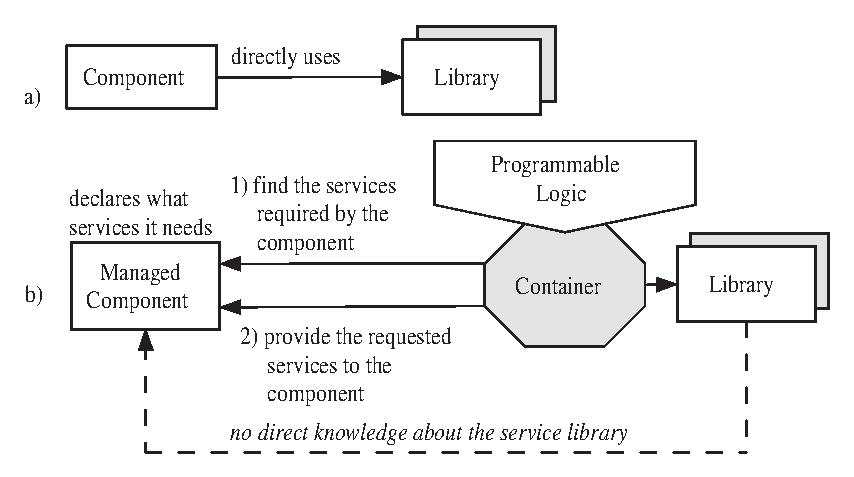
\includegraphics[width=10cm,height=!]{ch02/ioc}
	\end{center}
	\caption{Container Service Dependency Injection}
	\label{fig:con-inject}
\end{figure}

The lightweight coupling of a component with the container environment can be achieved using additional levels of abstraction. Instead of providing a component with direct access to the needed services, as in case (a) of \fig{fig:con-inject}, an agreed convention based on some form of \textit{inversion of control} \cite{fowler.ioc.04} abstraction can be used, as shown in the case (b) of \fig{fig:con-inject}. In case (b), the managed component only declares the services it needs, e.g., by using DSA constructs. The managed component does not have a direct knowledge of any particular service implementation. The container contains the functionality to provide the requested services to the component. The container implementation could provide only a predefined set of services, or the container can have programmable logic to be extended to provide arbitrary services \seec{ch05}.

The most interesting point in a container implementation is, thus, how to define abstractions for \textit{programmable dependency injection}, i.e., how to define dependencies of a managed component programmatically after the component has been created. Based on the terminology defined in \cite{java.compost}, this section distinguishes between \textit{invasive} and \textit{non-invasive} container implementation techniques and gives some examples for each case. Each of the discussed implementation techniques can be seen as a fine-grained variation mechanism.

\subsection{Non-Invasive Container Implementation Techniques}

Non-invasive container implementation techniques are based on pure object-oriented (OO) mechanisms mainly, interfaces, composition, inheritance and reflection. They do not need any special language support, and can be easily implemented in any existing OO language\footnote{Techniques for non OO languages also exist, but these languages will not be considered.}. In a non-invasive technique, there are no components / units more privileged than the others with respect to their power to access and modify other components / units. The entire component access goes through the declared (public) interfaces and uses only standard OO techniques, i.e., non-invasive techniques respect the OO encapsulation.

There are three main ways to inject component dependencies using non-invasive composition techniques: \textit{constructor injection}, \textit{setter injection}, and \textit{interface injection} \cite{fowler.ioc.04}. Almost all implementations of these techniques require reflective introspection support, i.e., internally they use some form of a reflection API. The discussion of non-invasive techniques in this section is based on \cite{fowler.ioc.04}. To demonstrate the \textit{constructor injection} and the other techniques, an example of a Java MIDP based game score class \cite{www.j2me} will be used, shown in \fig{c2f:gamescore1}. The example is made of a \texttt{Ga\-me\-Sco\-re} class, whose internal state needs to be saved in the local memory of a mobile device.

\begin{figure}[ht]
	\centering
	\begin{minipage}[b]{8.5cm}
	\begin{center}	
\begin{scriptsize}
		\begin{lstlisting}[numbers=left,language=Java,frame=leftline]{}
interface Serializer {
   public void Save(string id, byte[] data);
   public byte[] Load(id);
}

class RawSerializer() implements Serializer { ... }

class GameScore() {
   public GameScore(Serializer sr) {	...	}
	
   public void Save() {
      sr.Save(this.GetId(), this.GetData());
      ... 
   }
   ...
}	
		\end{lstlisting}
		\end{scriptsize}
	\end{center}
	\caption{GameScore Serialization Example}
	\label{c2f:gamescore1}
\end{minipage}	
\end{figure}

The \texttt{Se\-ria\-li\-zer} interface (lines 1 - 4) in \fig{c2f:gamescore1} declares operations for saving any data in the device memory, that can be represented as byte arrays. The \texttt{Raw\-Se\-ria\-li\-zer} class, in line 6, implements the actual serializing functionality. To keep things simple, it is assumed that the \texttt{Ga\-me\-Sco\-re} class contains two methods \texttt{Get\-Id()} and \texttt{Get\-Da\-ta()}, which return a string ID for the object (the key), respectively its data as a byte array (the value). An automatic implementation of the \texttt{Get\-Da\-ta()} method will be shown in \sr{ch2:inv}.

\begin{figure}[ht]
	\centering
	\begin{minipage}[b]{8.5cm}
	\begin{center}	
\begin{scriptsize}
\begin{lstlisting}[numbers=left,language=Java,frame=leftline]{}
class GameScore() {
   private Serializer sr = new RawSerializer();
   
   public GameScore() {	...	}
	
   public void Save() {
      sr.Save(this.GetId(), this.GetData());
      ... 
   }
   ...
}	
		\end{lstlisting}
		\end{scriptsize}
	\end{center}
	\caption{Direct Dependency Access}
	\label{c2f:direct}
	\end{minipage}	
\end{figure}

To demonstrate the constructor injection, the \texttt{Ga\-me\-Sco\-re} constructor expects an object implementing the \texttt{Se\-ria\-li\-zer} interface. The \texttt{Ga\-me\-Sco\-re} class can be connected directly to \texttt{RawSerializer}, as shown in \fig{c2f:direct}, which is equivalent in functionality and simpler to implement. This method would tie the \texttt{Ga\-me\-Sco\-re} implementation to the \texttt{Raw\-Se\-ria\-li\-zer} class. The connection between \texttt{Ga\-me\-Sco\-re} and \texttt{Raw\-Se\-ria\-li\-zer} is explicitly coded. The programmer decides about the exact implementation of serialization to use, at the time the \texttt{Ga\-me\-Sco\-re} class is coded. Thus, the direct connection is the least flexible dependency method.

\begin{figure}[ht]
	\centering
	\begin{minipage}[b]{12cm}
	\begin{center}	
\begin{scriptsize}
\begin{lstlisting}[numbers=left,language=Java,frame=leftline]{}
MutablePicoContainer pico = new DefaultPicoContainer();
pico.registerComponentImplementation(RawSerializer.class);
pico.registerComponentImplementation(GameScore.class);
GameScore gameScore = (GameScore) pico.getComponentInstance(GameScore.class);
gameScore.Save();
		\end{lstlisting}
		\end{scriptsize}
	\end{center}
	\end{minipage}
	\caption{Constructor Dependency Injection with PicoContainer}
	\label{c2f:pico1}
\end{figure}

%for all
\begin{dinglist}{43}

\item \textit{Constructor injection}. \fig{c2f:pico1} shows how the \texttt{Ga\-me\-Sco\-re} class of \fig{c2f:gamescore1} and the \texttt{Raw\-Se\-ria\-li\-zer} instances could be coupled programmatically using PicoContainer \cite{java.picocont}. PicoContainer assumes that the classes to be connected already define constructors for the appropriate service parameters. 
The \texttt{pico} container object contains all dependency information required to connect the \texttt{Ga\-me\-Sco\-re} and \texttt{Raw\-Se\-ria\-li\-zer} instances. To connect \texttt{Ga\-meSco\-re} with a new \texttt{Se\-ria\-li\-zer}, for example \texttt{Remo\-teSeria\-li\-zer} that can save data to a server when there is a network connection present, only the \texttt{Raw\-Se\-ria\-li\-zer.class} need to be replaced with the new \texttt{Remo\-te\-Se\-ria\-lizer\-.class} in the container. The PicoContainer indirection assures that \texttt{Ga\-me\-Sco\-re} will never know directly about a particular \texttt{Se\-ria\-li\-zer} implementation it is using. Having a \texttt{Se\-ria\-li\-zer} interface is not a requirement for PicoContainer. It can also connect instances of classes directly by examining their interfaces and finding the appropriate services based on the method signatures by using reflection. 

\item \textit{Setter injection} is similar to constructor injection, but makes use of the assumption that component classes implement appropriate setter methods for service components they depend on. In the example of \fig{c2f:gamescore1}, this could be accomplished by having the \texttt{Ga\-me\-Sco\-re} class define a \texttt{setSe\-riali\-zer(Se\-ria\-li\-zer sr)} method. A container implementation that relays mainly on setter injection is Spring Java / Java EE Application Framework \cite{www.spring}. There are several semantic differences between setter and constructor injection approaches. The setter injection provides more flexibility:
\begin{itemize}
\item An object can be created even though not all dependency objects it requires are available. This is not possible with the constructor injection, where all dependencies must be known when the object is created.
\item When using the setter methods, dependencies can be changed during the lifetime of an object. Often, a certain service needs to be attached to different existing instances and this is not possible with constructor injection. This can be useful, for example, when a virtual instance \cite{server.patterns.02} in an EJB container needs to be connected with a previously saved object state. With constructor injection, a new object must be always created, whereas with setter injection existing objects can be reused.
\end{itemize}
There are also some drawbacks that result from the flexibility of the setter injection:
\begin{itemize}
\item Given an existing component instance, it cannot be guaranteed that the instance is fully and properly initialized in the context of a container, or whether it needs more dependencies to be injected. Repetitive checks need to be performed every time an object instance is used to make sure that the dependencies are properly configured.

\item An explicit search must be carried out by the container to find the appropriate setter methods and decide for the right service objects to be passed, based on the setter method signature. This requires scanning the component interface for all possible methods, finding whether there are any setter methods, and matching the signatures of setter methods to the service components. Hence, the setter injection takes in average longer than the constructor injection. In the later, only the constructors need to be checked when new instances are created.
\end{itemize}

The setter injection is an example of what will be called a \textit{pseudo-syntax} convention to add custom semantics to a language \see{ch03.pseudo.syn} without changing its grammar. A pseudo-syntax construct is not an explicit part of the grammar syntax of the language. It is a \textit{coding convention} and is not checked by the compiler. In this case, the \textit{set} prefix is used as an implicit \textit{syntactic pattern} to define the setter injection. 

\item \textit{Interface injection} is a generalization of the setter injection. Instead of having required constructors or setter methods in the game score example, an interface \texttt{In\-ject\-Se\-ria\-li\-zer} with a single method \texttt{in\-jectSe\-ria\-li\-zer(Se\-ria\-li\-zer sr)} is defined, and the \texttt{Ga\-me\-Sco\-re} class will implement it. Based on the \texttt{In\-jectSe\-ria\-li\-zer} interface, an interface injection container implementation can couple the object and the service\footnote{The reader is referred to \cite{fowler.ioc.04} for an example of a framework that uses interface injection.}.

The interface injection pattern has the same benefits and drawbacks as the setter injection.
However, interface injection improves the search by making the injection points explicit. The container needs to search only for the implemented interfaces and their methods to find what services need to be provided to a given component. No pseudo-syntax checks are required, such as, the check for the \textit{"set"} method prefix. Adherence to pseudo-syntax constructs cannot be checked at the compile-time. Hence, employing pseudo-syntax constructs as a mean of interfacing with the dependency container is more error prone that using interfaces for the same purpose. Pseudo-syntax checks rely also extensively on string pattern matching, which is a resource consuming task when done repeatedly at run-time.

When interfaces are used to denote custom semantics by tagging class implementations, they are known as \textit{marking interfaces} \cite{design.attrib}. The interfaces that require trivial method implementations just for the sake of service injection will be treated as marking interfaces here. In an invasive container \see{ch2:inv}, a marking interface does not need to contain methods that must be implemented in the classes that use the interface. An invasive container can modify a component decorated with \texttt{In\-ject\-Se\-ria\-li\-zer} interface to properly inject the required serialization service. In non-invasive containers marking interfaces may contain methods. 

Marking interfaces can be used to add semantics to components in languages that do not provide explicit attributes, such as, Java 1.4 \cite{www.java,java.attrib4j}. They can be used to declare dependencies, as in the case of injection pattern, or other properties that a component must have\footnote{A well-known example is the use of the \textit{Se\-ria\-li\-zable} interface in Java. Another example is the \textit{Null Object} pattern \cite{refactor.99}, where a class defines specific functionality for the null case by using inheritance from a Null (marking) interface.}. Marking interfaces have also some problems. As \kr{ch03} discusses, the number of marking interfaces can grow exponential in a system, in the case when interfaces are used to support component variability.

\end{dinglist}

There are also several other non-invasive techniques, less flexible than the ones explained above. They are used less frequently to implement the dependency indirection in a container. Only \textit{service locator} \cite{fowler.ioc.04,j2ee.without.ejb.04} and \textit{mix-ins} \cite{bracha90mixinbased,Ernst.99,flatt98classes,Duggan.00} will be briefly considered in this section.

\begin{dinglist}{43}

\item \textit{Service locator} makes service acquisition explicit. The idea is to locate the services of interest explicitly by consulting a (well-known) object registry. The registry location could be hardwired in the component implementation, or it can be indirectly passed to it using any of the above dependency injection techniques. In the service locator case, the  \texttt{Ga\-me\-Sco\-re} example would contain code to get the serializer object directly from the object registry as in \fig{c2f:locator}. Any directory (LDAP\footnote{Lightweight Directory Access Protocol.}), trading, or naming service can be used as a locator repository for objects. The locator must find the required service object and properly initialize it. The requested registry object path (e.g., a relative path \textit{"Lo\-cal\-Se\-ria\-li\-zer"}, or an absolute path \textit{"jndi://mobcon/services/LocalSerializer"}) can be hard coded in the application, or read from a configuration file.

\begin{figure}[ht]
	\centering
	\begin{minipage}[b]{12cm}
	\begin{center}	
\begin{scriptsize}
\begin{lstlisting}[numbers=left,language=Java,frame=leftline]{}
ServiceLocator locator = ...
LocalSerializer s = (LocalSerializer)locator.loadService("LocalSerializer");
		\end{lstlisting}
		\end{scriptsize}
	\end{center}
	\caption{Constructor Dependency Injection with a Service Locator}
	\label{c2f:locator}
	\end{minipage}	
\end{figure}

The service locator offers less automation than the other techniques presented above. Finding services is explicitly encoded, and the kind of service the programmer is asking for, must be exactly know \cite{j2ee.without.ejb.04}. Furthermore, service locator adds accidental complexity to the component's implementation. The service locator is sometimes used as a complementary technique to other dependency injection mechanisms in a system. For example, JNDI \cite{www.jndi} is used in Java EE to access secondary application resources, e.g., images and Java Server Pages (JSP).

\item \textit{Inheritance and Mix-ins} can also be used to emulate indirect dependencies \cite{dip}. Mix-ins \cite{bracha90mixinbased,Ernst.99,flatt98classes,Duggan.00} factor out properties that cross-cut more than one class \cite{riel.96}. In the particular case of the containers, a mix-in can contain the context for a container service. Mix-ins can be implemented using multiple-inheritance, or with templates in the languages that support them \cite{SmaragdakisBatory.02,generative.00}, e.g., with C++ templates, or Java generics.

The inheritance based techniques are usually static\footnote{There are also exceptions, e.g., Rondo \cite{rondo.97}.}, i.e., static linking (deployment) of components is required. For this reason, inheritance composition techniques are usually less flexible than other non-invasive techniques. No known container implementation exists that relies exclusively on inheritance techniques. The mix-ins technique appears often in different forms in different systems \cite{genvoca.94}, which is why it was discussed as an separate alternative here.

\end{dinglist}

\subsection{Invasive Implementation Techniques}
\label{ch2:inv}

%Invasive techniques access the implementation of a component directly, usually relying on the Abstract Syntax Tree (AST) of a program, ignoring the declared (public) interface of the component or making use of the knowledge about the components internal implementation details.

If a container is considered to be a strict component system in the OO sense, then only the non-invasive techniques make sense. They respect the integrity of individual components and operate in accordance with the OO encapsulation rules. A container in this case contains non-invasive code to connect the application components with the container predefined services (other well-known components). The container services are just other components. A well-designed container (non-invasive, or invasive) is usually extensible, i.e., new service components may be added.

Another view of a container is as a transformation system\footnote{The term \textit{transformation} is used here to include any generation or transformation technique that requires some form of AST, or equivalent program structure, processing. Sometimes, the same technique can be supported with generative techniques, or with run-time support. No distinction will be made between the two techniques. The run-time support will be considered to be a specialized optimization.}, much like a compiler / transformer. In this case, the components used inside the container environment need to be somehow transformed, so that the expected dependencies are injected into their inner implementation. The container in this case is a programmable transformer, whose input consists of the components, container services (other well known components), and a specification how to connect the first two with each-other. The specification can be given explicitly in some particular syntax, or it can be implicitly inferred from the implementation of components. The details of the specification are used to create \textit{the glue code} \cite{halloway.02} that connects the components with services. The output of such a transformation is a system, where the components and the services are properly connected with each-other by conventional OO mechanisms.

\textit{Invasive techniques} support the transformation view of a container. Invasive techniques require either special language features\footnote{Such as, the ability to access and (arbitrarily) manipulate the source AST, or the run-time meta-model of the program.}, or external frameworks that provide means to mutate the internals of a component, surpassing the usual OO techniques. Invasive source code or binary mutations may not be directly supported by the target language, in which the original component is written. Invasive techniques do not respect the OO encapsulation and depending on the implementation, they can change a component arbitrarily.

An invasive technique can introduce changes to the component internals, or just read the component internals to introduce non-invasive changes \see{attrib.trans}. That is, the invasive techniques can be \textit{read-only} or \textit{read / write}. Read-only invasive techniques can be treated as non-invasive. However, the read-only invasive techniques will be classified as invasive here, because they require access to component internals which are not visible through the declared interface of the component. An example is the use of the Reflection API in Java. By default, the Reflection API  returns only the public members of a class, and is non-invasive by the definition. The private methods can be accessed by changing member access permission by using the \texttt{Reflect\-Permi\-ssion} class. This latter case will be treated as a form of the read-only invasive access to a class.

A distinction is made in \cite{java.compost} between invasive techniques that use \textit{explicit} and \textit{implicit} \textit{hooks}. A \textit{hook} is defined as an accessible point of the component interface or implementation that can be used to modify the component and to inject code into it. Explicit or declared hooks are hooks that are defined explicitly by the programmer to indicate that the code associated to them will change. An example would be the decoration of a method with an attribute, or a special predefined prefix in its name. Implicit hooks can be any accessible point of a component, even those that are not foreseen by the original developer, e.g., a method call at run-time.

Accessible points of a component depend on the technology used to access the description of the component's implementation. Not all technologies are equally expressive. For example, method internals cannot be accessed using OO reflection alone. Therefore, the code inside a method cannot serve as a hook when the reflection technology is used. The term \textit{hook} will not be used here anymore, because it is also used to name some special callbacks in event-driven applications. The term \textit{hook} in \cite{java.compost} is more or less used with the same meaning as the term \textit{joinpoint} in Aspect-Oriented Programming \cite{kiczalesetal.97}, which is more specific and will be used in this chapter. Joinpoints will be further discussed in \sr{ch2:aop}.

Any system that supports some form of access and manipulation of the abstract syntax tree (AST), e.g., JTS \cite{batory98jts}, can be used to implement invasive containers. Invasive techniques will be illustrated here by an example which uses syntax similar to COMPOST~\cite{java.compost}.

\begin{dinglist}{43}

\item \textit{Invasive Example.} The service dependency injection in the \texttt{Ga\-me\-Sco\-re} example of \fig{c2f:gamescore1} could be easily implemented with invasive techniques. The AST of the \texttt{Ga\-me\-Sco\-re} class needs to be traversed to add / modify the serialization service variable and make it point to the requested service. Given that this case is trivial, the example will rather show how the \texttt{Get\-Da\-ta()} method of the \texttt{Ga\-me\-Sco\-re} class could be implemented with invasive techniques. This method returns a byte representation of a \texttt{Ga\-me\-Sco\-re} object's state. 

The example of the \texttt{Get\-Da\-ta()} method implementation is more interesting, because it shows how the invasive techniques can be used to introduce functionality inside a method. This is impossible to realize directly with non-invasive techniques. Part\footnote{To keep the discussion simple, it is assumed that the \texttt{Ga\-me\-Sco\-re} class includes only simple primitive types. Object serialization should follow the containment dependencies to properly serialize all field objects. Checking of the special cases is also omitted from the code.} of the implementation of the \texttt{Get\-Da\-ta()} method is illustrated in \fig{c2f:getdata}, by using pseudo-syntax similar to the one found in COMPOST \cite{java.compost}.

\begin{figure}[ht]
	\centering
	\begin{minipage}[b]{12cm}
	\begin{center}	
\begin{scriptsize}
\begin{lstlisting}[numbers=left,language=Java,frame=leftline]{}
CompilationUnitBox box = 
    compositionSystem.createCompilationUnitBox("GameScore.java");
List<FieldBox> fields = box.findField("*");
//<<check if there are fields>>
MemodBox method = compositionSystem.createMethodBox("GetData");
//<<specify method parameters, scope and return type>>
//<<add code to the method to init an in-memory binary writer>>
for(FieldBox field : fields)
{
    method.addString("binaryWriter.Write(" + field.Name + ");\n");
}
//<<add code to method to properly return bytes from binaryWriter>>
box.addMethodBox(method);
		\end{lstlisting}
		\end{scriptsize}
	\end{center}
	\caption{The Invasive Implementation of the \texttt{GetData()} Method}
	\label{c2f:getdata}
	\end{minipage}	
\end{figure}

All the member fields of \texttt{Ga\-me\-Sco\-re} class are accessed, and based on them the code for a new private method \texttt{Get\-Da\-ta()} is generated. \texttt{Get\-Data()} serializes the data of each field in a memory binary stream. The example of the \fig{c2f:getdata} accesses first the Java class (GameScore.java) and implicitly parses it in lines 1 - 2. Then, it builds a list of all fields found in the input class (line 3). It creates a new method node (line 4) for the \texttt{Get\-Da\-ta()} method that needs to be added. The details of the method node, such as its return type and the parameters, are specified in lines 6 - 7 (not shown). The example traverses over all the fields which are found in the fields list. For each field, code to serialize its contents into a series of bytes is added to the new \texttt{Get\-Data()} method (lines 8 - 11). Finally the created method is added to the class (line 13)\footnote{The code which saves back the class after its modification is omitted.}. 

A similar method \texttt{Set\-Da\-ta(by\-te[]\- data)} that reverses the serialization process could also be generated at the same time.

\end{dinglist}

While a Java source code unit (*.java) is shown in this example, the input could also be a compiled Java class (.*class). The class file (bytecodes) can be processed either at load-time or at run-time if the particular invasive system has the support for that.

As illustrated by this example, even for relatively small tasks, invasive compositions require tedious coding. This is an inherent property of API-based generation systems \cite{voelter.generation} due to the programming indirection. Rather than writing the source code directly, code that generates the code is written. The indirect code has also to deal with each special case.
%
Code templates and textual pieces of code can be used to shorten the amount of code that needs to be written programmatically and debugged indirectly. The \texttt{Get\-Da\-ta()} method could also be created from a predefined source code template. The template would then be bounded \cite{java.compost}\footnote{That is, template parameters will be replaced by the specific code for the use-case.} to the specific code generated to serialize each field. Suitable predicates, which are used to control the AST node selection and iteration, as those in \cite{trans.strategy.01}, can also reduce the needed work.


\subsection{Non-Invasive versus Invasive Techniques}

Most software composition problems, such as the dependency injection, can be solved either with non-invasive or invasive techniques. However, there are several differences between the non-invasive and invasive techniques with regard to:

\begin{itemize}
\item \textit{Automation} - invasive techniques help to achieve more automation, because they can be customized for the problem at hand. Invasive techniques reduce better the accidental complexity of the solution.
\item \textit{Flexibility} - invasive techniques are more flexible for making changes inside components. Invasive changes are either not possible with non-invasive techniques, or require many explicit indirection layers to be implemented. 
\item \textit{Dynamicity} - non-invasive techniques enable changing the binding of the components with services at the run-time. Invasive techniques are static: they usually operate over the AST of a program. Invasive techniques could also be implemented dynamically when appropriate run-time support is provided.  %streamloom example
\item \textit{Ease of the implementation} - non-invasive techniques require only OO mechanisms which are found by default in many languages. Invasive techniques require meta-language extensions or external frameworks that need to be maintained explicitly as the core language changes.
\end{itemize}

Depending on the particular properties of the specific systems, sometimes dynamicity is preferred to flexibility and automation, and sometimes using existing language support is preferred to using external frameworks. For mobile containers, the declarative language constructs are supported with attributes, so that the static invasive techniques make more sense. Maximum automation is needed and the generic dynamicity of non-invasive compositions is not required in the addressed MIDP \cite{www.midp-ota} systems \seec{ch05}. \Sr{sec:var.mob.pl} listed several preferable properties of the variability mechanisms for mobile product-lines. Table~\ref{tab:InvasiveVSNonInvasive} summarizes how these criteria are supported by invasive and non-invasive techniques, in the context of attribute enabled mobile product-lines.

\begin{table}[ht]
	\begin{center}
		\begin{tabular}[t]{|l||l|l|}
\rowcolor[gray]{.7}
\hline
Criteria & Invasive & Non-Invasive \\
\hline
Explicit programming model, possibly DSL based & + & - \\
Enable automation & + & - \\
Low start-up / evolution costs & - & + \\
Domain-specific optimizations & + & - \\
\hline
		\end{tabular}
	\end{center}

	\caption{Techniques for Attribute Mobile Containers - Invasive versus Non-Invasive}
	\label{tab:InvasiveVSNonInvasive}
\end{table}

As shown in Table~\ref{tab:InvasiveVSNonInvasive}, invasive techniques can be used to support an explicit programming model with DSA at the language level. The focus is in the invasive interpretation of explicit joinpoints modeled with attributes. Invasive techniques can be used to automate attribute-based DSA transformation and also to process implicit joinpoints \see{ch2:aop}. Explicit attributes, combined with invasive techniques, help to reduce the accidental complexity of the programming model. The last line of Table~\ref{tab:InvasiveVSNonInvasive} shows that, for mobile containers, invasive techniques also support better the optimizations, e.g., specific selection of service code, or reduction of the abstractions being used.

The only benefit of non-invasive techniques with regard to the criteria in Table~\ref{tab:InvasiveVSNonInvasive} is that they do not require any special language support and have lower start-up costs. That is, non-invasive containers are easier to implement.
However, non-invasive techniques do not support an explicit declarative programming model. This means that more lines of code need to be written with non-invasive techniques. Therefore, non-invasive techniques offer less automation than invasive ones. Appropriate lightweight attribute-based DSA technology can help to reduce the startup costs of invasive DSA techniques and to preserve the DSA automation benefits.

Invasive techniques have several liabilities that need to be addressed:

\begin{itemize}
\item \textit{Lack of language technology support.} Invasive techniques may not be directly supported by the language. Source-to-source transformers require access to the AST of the component code. For languages that support binary meta-data, such as Java \cite{www.java}, transformations at binary level can be used. Some equivalent of source code AST is preserved and need to be accessed and manipulated.  Not all OO languages offer such AST access as part of their libraries. Third-party parser tools need to be used. These tools should be explicitly maintained when the target language changes. Third-party meta-programming frameworks increase the overall cost of the container implementation\footnote{For example, third-party tools used to parse Java code or manipulate Java binaries have difficulties moving from JDK 1.4 to JDK 1.5. JDK 1.5, introduced a lot of new syntax and the binary meta-data were slightly enriched. The Java vendor (Sun) does not support any transformation interface for Java binaries.}, and could result in higher costs for a product-line, as compared to the non-invasive techniques. 

\item \textit{Transformation side-effects.} The flexibility of invasive techniques raises new problems for debugging and traceability. Transformation side-effects\footnote{For example, joinpoint matching with pointcuts in AspectJ \cite{www.aspectjt} may match also program elements that were not intended as the system evolves.} may not be predictable in all cases. Despite of the flexibility of invasive techniques, developers need to be conservative in the way they use them (the so-called \textit{sound} compositions in \cite{java.compost}). Explicit extension points, used in frameworks and explained in \sr{sec:ooframeworks}, can be combined with the invasive techniques to narrow the range of transformation possibilities in a product-line and reduce the transformation side-effects.
\end{itemize}

\section{Aspect-Oriented Programming and Product-Lines}
\label{ch2:aop}

The transformations of attribute-based DSA \see{c2.sec.dsa.attributes} that are presented in this book can be supported with any generic invasive meta-programming system. This section discusses Aspect-Oriented Programming (AOP) \cite{kiczalesetal.97} as a generic technique that can be used to support invasive compositions. AOP is used to implement horizontal\footnote{Horizontal transformations have both the domain and the co-domain in the same MOF \cite{www.mof} level. Vertical transformations have the domain and the co-domain in different MOF meta-levels.} transformations \cite{sf.04} within the same system meta-level, usually within a single programming language. Arbitrary meta-program generators and DSA can be used to implement horizontal, but more often vertical transformations, which cross more than one meta-level \see{sec.aop.dsa}. There is an overlap of various program transformation technologies that affects also attribute-based transformations. Attributes can be used to carry either horizontal, or vertical  semantics and serve as a bridge that enables AOP engines, which can access attributes, e.g., AspectJ \cite{Laddad.aop, www.aspectjt}\footnote{With support for Java 1.5 annotations.}, to support vertical transformations that can be expressed with attributes. 

This overlap has several consequences. More than one technology can be utilized to achieve the same transformations. All AOP examples given in \cite{Laddad.aop}, can be equally solved with any invasive transformation framework, even though some more explicit context book-keeping data may be occasionally needed. For example, the AOP techniques could be explained in terms of hooks in the COMPOST \cite{java.compost}, a generic invasive composition system. It is, thus, often not clear when to choose one technology or another. There is also no clear boundary on the limits of what can be achieved with specific technologies, such as AOP.

This section elaborates more about the position of AOP for supporting generation. AOP techniques will be compared with DSA in \sr{sec.aop.dsa}. This section considers AOP from a technical point of view as an invasive transformation technique. While the focus will be on attribute transformations, much of the discussion in this section is general and applies not only to mobile product-lines.

\subsection{Introduction to AOP Techniques}
\label{sec:aop-intro}

Aspect-Oriented Programming (AOP) \cite{kiczalesetal.97} comprises a set of technologies aimed at better modularization of cross-cutting concerns found in software systems. This section discusses AOP from a technical perspective. The interest will be in the transformation mechanisms used by AOP and not in the modularization issues \cite{Crosscutting2.03}. %We will introduce first the AOP technology and terminology. 
The discussion of AOP technology is based mainly on the AspectJ programming language \cite{Laddad.aop, www.aspectjt}\footnote{AspectJ is Java dialect with AOP extensions. The AspectJ's predicate model has been influential to other AOP languages.}. The scheme in \fig{fig:ch2aop} illustrates the relations between the main components found in AOP terminology.

\begin{figure}[ht]
	\begin{center}
		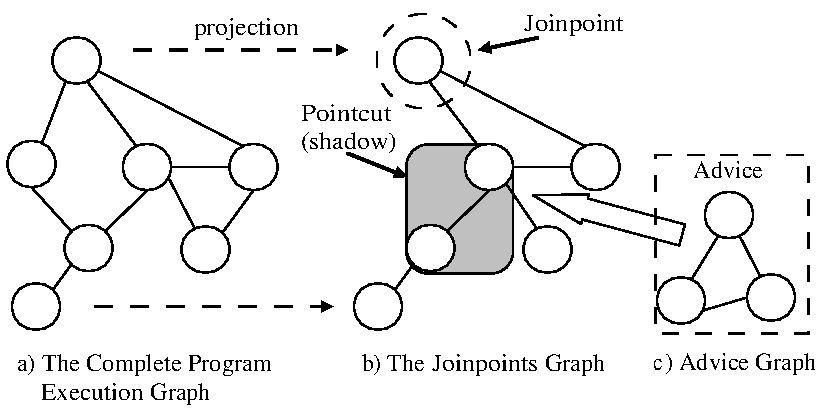
\includegraphics[width=12cm,height=!]{ch02/aop}
	\end{center}
	\caption{Illustration of Components found in the AOP Terminology}
	\label{fig:ch2aop}
\end{figure}

\begin{itemize}
\item A program is seen in AOP as an \textit{execution graph} \cite{aop.modeling.03}. A node in this graph represents a possible state of the program and an edge represents a transition from one state to another. The node set of the execution graph of a program includes theoretically any state in a program execution, with all possible paths to that state from the other states as shown in part (a) of \fig{fig:ch2aop}.

Building the complete execution graph for any arbitrary program and any possible input is unfeasible. The term \textit{execution graph} is often used in AOP to mean some abstraction of the entire execution graph, consisting of some representation of the Abstract Syntax Tree (AST) and eventually augmented by information from additional static or dynamic analysis, e.g.: data flow information, control flow information, and other forms of execution history. Collecting the additional information, e.g., execution history, may require special run-time support\footnote{An optimization used in  AspectJ \cite{www.aspectjt} is to simulate part of execution to collect some run-time data from the static AST to avoid the overhead of run-time support, for example, when implementing \textit{cflow}.}.

\item Accessible points of the execution graph are called \textit{joinpoints} and are defined as \textit{"any identifiable execution point in a system"} \cite{Laddad.aop}.
%
As shown in part (b) of \fig{fig:ch2aop}, joinpoints are a subset of the execution graph accessible in a particular representation of it\footnote{A projection in time and space of the execution graph.}. A joinpoint model describes the execution graph nodes based on the context where they are found, shown as edges inside the dashed circle in part (b) of \fig{fig:ch2aop}. That is, the execution nodes are identified not only by their own characteristics, e.g., a method signature, but also from the context where they exist, e.g., where the method is being called.

As mentioned in \sr{ch2:inv}, the accessible points of a program graph depend on the technology used to describe it. Some systems, such as AspectJ, place further restrictions on accessible joinpoints and distinguish between all possible joinpoints (accessible for example thought AST) and \textit{exposed} joinpoints \cite{Laddad.aop}. For example, AspectJ's joinpoint model does not expose loops. That is, loops are a possible, but non-exposed joinpoint.

\item An execution graph is a state machine. To modify the execution graph, there should be a way to select sets of nodes of interest and modify, replace, or delete them. There are two ways how this can be done and both are explored in AOP:

\begin{enumerate}[i.]
\item The execution graph is totally known\footnote{This is of course not possible all the time, especially at run-time.}. That is, the entire state machine graph, or at least the wanted parts to change, are known. In this case, it can be spoken of \textit{selection} of nodes and of explicit \textit{search} over the execution graph. Depending on the execution graph representation, many transformations are possible in this total view. For example, often the AST is used as a representation of the total execution graph.
 \item The execution graph is partially known at run-time. Transformations over the total view of the execution graph cannot be done in real-time. This could be a problem for those graph transformations that rely on information that is available only at run-time. In this case, the execution graph can be seen as an automata, and the transformation process can wait for patterns of transitions to appear, or \textit{events}. Every time an event happens, a respond to it in real-time with predefined \textit{event handlers (callbacks)} can be programmed.
\end{enumerate}

The real-time processing of events\footnote{That is, responding to the events as soon as they happen with the allowed timespan.} requires some form of run-time support which is often not acceptable, because of the additional overhead, or proprietary technology additions. Using partial evaluation \cite{jonesetal.93} (partial execution) techniques, many real-time (dynamic) events can be equally expressed statically, by using the information found in total static models, such as the AST, the way AspectJ does. The total view of the graph is preferable, as it removes the need to maintain the execution context. The real-time partial view requires maintaining the execution context explicitly\footnote{This is analogous to the difference between DOM and SAX parser models for XML documents (http://www.w3.org/) \cite{mcl.01}. A \textit{Dynamic Object Model (DOM)} parser processes entirely an XML document and builds a total tree of its nodes, so the node tree can be explicitly searched and modified using XPath or XQuery. A \textit{Simple API for XML (SAX)} parser, on the other hand, generates events (that can be processed as necessary) every time it encounters a node tag in a XML document. In the SAX parsers case, the context, where a node is found with regard to the other nodes, needs to be maintained explicitly when needed.}.

AOP systems logically use the real-time event-based way for reacting to sets of nodes of interest. Practically, most events can be statically implemented. For this reason, some of the early AOP systems, such as AspectJ, speak about \textit{virtual events} over the program control flow \cite{Laddad.aop}. Newer implementations, especially those of dynamic AOP, such as Prose \cite{prose}, react to actual events in the program execution and the distinction between virtual events and event-driven (triggered) systems is blurred. 

The event patterns of interest, over the execution graph, are made declarative by using specialized predicates. A predicate model could support the composition of primitive predicates. Predicates can be made part of a general-purpose language, and are known in AOP as \textit{pointcuts}. For example, pointcut predicates, such as \textit{cflow}, are made part of the AspectJ syntax. The selection criteria in a pointcut is based on all characteristics of a joinpoint, this includes a node in the execution graph and its context.

\item Every time an event of interest is matched by a pointcut predicate, some action of interest (event handler) can be executed. This is known as \textit{advice} in AOP and is shown in part (c) of \fig{fig:ch2aop}. The execution graph regions matched by a predicate are also known as the \textit{pointcut shadow} \cite{aop.semantics.02}.

The advice contains code to be executed for the matched nodes. The modifications that the advice code can do to the execution graph can include any graph rewriting \cite{mens.99} technique, depending on the model used to present the execution graph.

The process of injecting the advice code into the pointcut shadows is known as \textit{weaving}. Depending on the AOP system the weaving process can be either static or dynamic.

\item The combination of pointcuts and advice is known as an \textit{aspect}. Depending on the particular system, an aspect may contain also other elements. For example, AspectJ aspects contain compile-time directives for errors, introduction (invasive changes in the structural hierarchy of a program), and can declare new methods and fields. 
\end{itemize}

\subsection{AOP as a Generic Invasive Transformation Technique}
\label{sec:aop-inv}

The above discussion about AOP shows that AOP engines are generic transformation engines, that can be used to carry out a great range of invasive transformations. AOP techniques have been used to support product-line variability \cite{foa-aop.04,framed.aspects}. The possible AOP transformation are limited only by the joinpoint model supported by a specific AOP engine implementation. The use of generic AOP engines, such as AspectJ, is preferable for program transformation because of:

\begin{itemize}
\item \textit{Language integration}. AspectJ is tightly integrated with the Java language. This enables a great range of compiler-based static checking to find errors in the aspect code\footnote{AspectJ is not the only generic generative framework that is statically checked.}.
   
\item \textit{Declarativenes}. AspectJ offers a set of declarative context-enabled predicates (pointcuts) to select nodes of interest\footnote{AspectJ users are not explicitly aware that aspects rely on the meta-model of a program to manipulate it. This is explicit in other systems with meta-programming capabilities.}. The pointcuts not only ease the implementation, they also build a common vocabulary to speak about node selection.
\item \textit{IDE support}. Statically checked generative tools with IDE\footnote{Integrated Development Environment.} support simplify the implementation of program transformations. AspectJ is tightly integrated to Java, and well supported by development tools, such as,  Eclipse AJDT \cite{Eclipse.AJDT}.
\end{itemize}

These features make any generic transformation system, such as AspectJ, preferable, because the cost of developing custom transformation systems is often high and cannot be justified. There are also several liabilities:

\begin{itemize}

\item \textit{Specialized transformation engines can explore better the domain characteristics.} Generic transformation engines, including the AOP ones, are not always the best option. Generic transformation engines could be used to implement transformations in those systems where it makes no sense to invest in a more specific transformation technology. However, invasive transformation frameworks specialized for a narrower purpose are better suited in the long term than any generic transformation engine. An example, where a specific technique is better suited than any generic technique, would be to add OO support to ANSI C. Starting with a C \texttt{struct} construct, additional abstractions around it could be defined, using a combination of C code and generative transformations as in \cite{ooc}, to make the \texttt{struct} construct behave as a C++ class. Any invasive transformation tool that allows us to access the AST of a C program can be used for this purpose. However, the complexity of the solution would make any generic tool based implementation complex. Specialized generative techniques for this problem, as in \cite{ooc}, work better in ANSI C case. And it is even better, when the OO abstractions are made part of the language, as they are in C++.

\item \textit{Limitations in transformation capabilities of generic systems.} Another issue with generic transformation engines is their transformation limitations. The limitations are unfortunately not always clearly stated. For example, the joinpoint model of AspectJ cannot be used to enforce capital name conventions \cite{aop.paradox.03}. These limitations exist on purpose in AspectJ. They make its programming model simpler and AspectJ was originally intended to make various modularization factorizations over the meta-model of a Java program easier. Supporting very detailed joinpoint models is possible, but would remove much of the declarativeness of the pointcut notations used. 

\item \textit{Limited support for vertical transformations.} AOP engines, such as AspectJ are tightly connected to the meta-model of the language they target. They cannot support new keywords or new language constructs. This makes some generic AOP systems, such as AspectJ, to offer limited support for implementing arbitrary DSA constructs. \Sr{sec.aop.dsa} returns to this issue and explains in more detail the relation between AOP and DSA.

\end{itemize}

\noindent \Kr{ch04} develops a transformation technology specialized for interpreting DSA emulated with attributes. Having a special transformation technology for this domain, enables developing modular attribute-driven transformers that are difficult to structure and enforce with more generic transformation technologies. It makes sense to invest on an attribute-driven transformation technology, as the problem is relatively complex,  very specific, and the attribute-driven transformation technology can be used to support open container frameworks to organize assets of product-lines for more than one domain. %In AOP terms, the domain-specific modularizations of \kr{ch04} specialize the organization of the advice code.

\cendsection{Chapter Summary}
\label{ch2sum}

%Several technologies exist for the mobile device application development. Virtual machine abstractions, e.g., J2ME MIDP, hide the complexity of the underlying hardware and specific operating systems. Developing automation mechanisms for specific mobile domains can help to further reduce the costs of mobile device applications.

More mobile device applications can be build and debugged in time, when product-lines are introduced. Iterative mobile application product-lines automatically reuse the common functionality of the mobile application families. Several variability mechanisms can be used to support mobile product-lines, e.g., OO libraries, frameworks, visual modeling with CASE tools, and domain-specific abstractions (DSA). 

DSA support the architecture of a mobile product-line at the language level, blur the architectural distinction between visual CASE tools and programming language constructs, and allow for domain-specific optimizations. The cost of introducing DSA remains still very high, and low-cost implementation mechanisms need to be explored. 

Software containers offer an convenient architectural pattern to organize product-line assets. Containers clearly separate the application specific functionality from the cross-cutting domain functionality. Containers can be used to transparently inject the domain services into a specific application. A mobile container is used to support product-lines for mobile device applications. The assets of a mobile product-line are organized as container services, having both a server and a mobile client part. DSA, combined with the container abstraction, can be used to create open container families for supporting iterative product-line development.

There are several invasive and non-invasive approaches to implement the dependency injection of services in containers. Non-invasive techniques are easier to implement, but offer less automation. Invasive techniques are better suited to support attribute-based DSA in mobile containers. Static invasive techniques, in the context of a container, can be used to bind the attribute-based DSA to the product-line services.

The need for several technologies was identified, that will be explored further in the following chapters:

\begin{itemize}
\item \textit{Lightweight language extensions based on attributes.} Attribute enabled language tech\-no\-lo\-gy can be used to emulate embedded DSA. Attributes support iterative product-line development with minimum start-up costs. Language technology that directly supports attribute-based transformations is needed \seec{ch03}.

\item \textit{Attribute-driven transformation support.} Any generic invasive programming technology can be used to implement and support attribute-based abstractions. Specialized transformations could help to better modularize attribute-based transformers and make them declarative. Attribute-based transformer technology enables the reuse of transformation components and declarative composition of attribute-based transformers \seec{ch04}.

\item \textit{Open container families.} Extensible containers are needed to organize the common mobile device application functionality. Mobile containers are specialized to address the peculiarities of mobile applications and to organize the mobile product-line assets, such as, the need for data adaptation \seec{ch05}.

\end{itemize}
